% !TEX root = ../rawlik-phd-thesis.tex
\chapter{Next-generation active magnetic shielding}
\label{ch:sfc-prototype}

The coil design method described in the previous chapter opened the door to a next generation of active magnetic shields, where the coil system is not much larger than the fiducial volume and where high-order terms of the magnetic field can be compensated, all while retaining a low number of controlled degrees of freedom.

In a laboratory at ETH Zürich an active shield was constructed.
In its first version it featured three coils for the homogeneous components of the magnetic field. The coils were wound on a regular grid.
Mapping of the magnetic field created by the coils confirmed that they produce a field at the specified homogeneity in a large volume.
The active shield was tested with strong, inhomogeneous disturbances, as well as its long-term stability.

A next iteration of the active shield was constructed on a grid with one open face.
This not only eased access to the inside, but also demonstrated coils of a more complicated design.

Finally, coil design for an active magnetic shield for the n2EDM experiment is proposed.
Despite tight spatial constraints, it achieves homogeneity of \SIrange[range-phrase=--,range-units=single]{1}{2}{\percent} around the mu-metal shield.




\section{The first iteration --- coil structure}
In the discussion of the coil design method a practical way to realise it was indicated---to construct a grid out of cable channels.
At ETH Zürich a system pictured in Fig.\,\ref{fig:prototype_photo} was built consisting of a $5 \times 9 \times 5$ grid of square tiles. Each tile had side length \SI{262}{\milli\meter}, the total size was $1310 \times 1310 \times \SI{2358}{\milli\meter}$.
The vertical axis we refer to as $z$, the long horizontal one as $y$, and the remaining axis $x$. The support frame was made of aluminum construction profiles.
To support the cable channels, on each side there was a large one-piece aluminum sheet, with square cut-outs leaving material only directly below the cable channels.
The plastic cable channels were glued onto the aluminum.

\begin{sidewaysfigure}
  \centering
  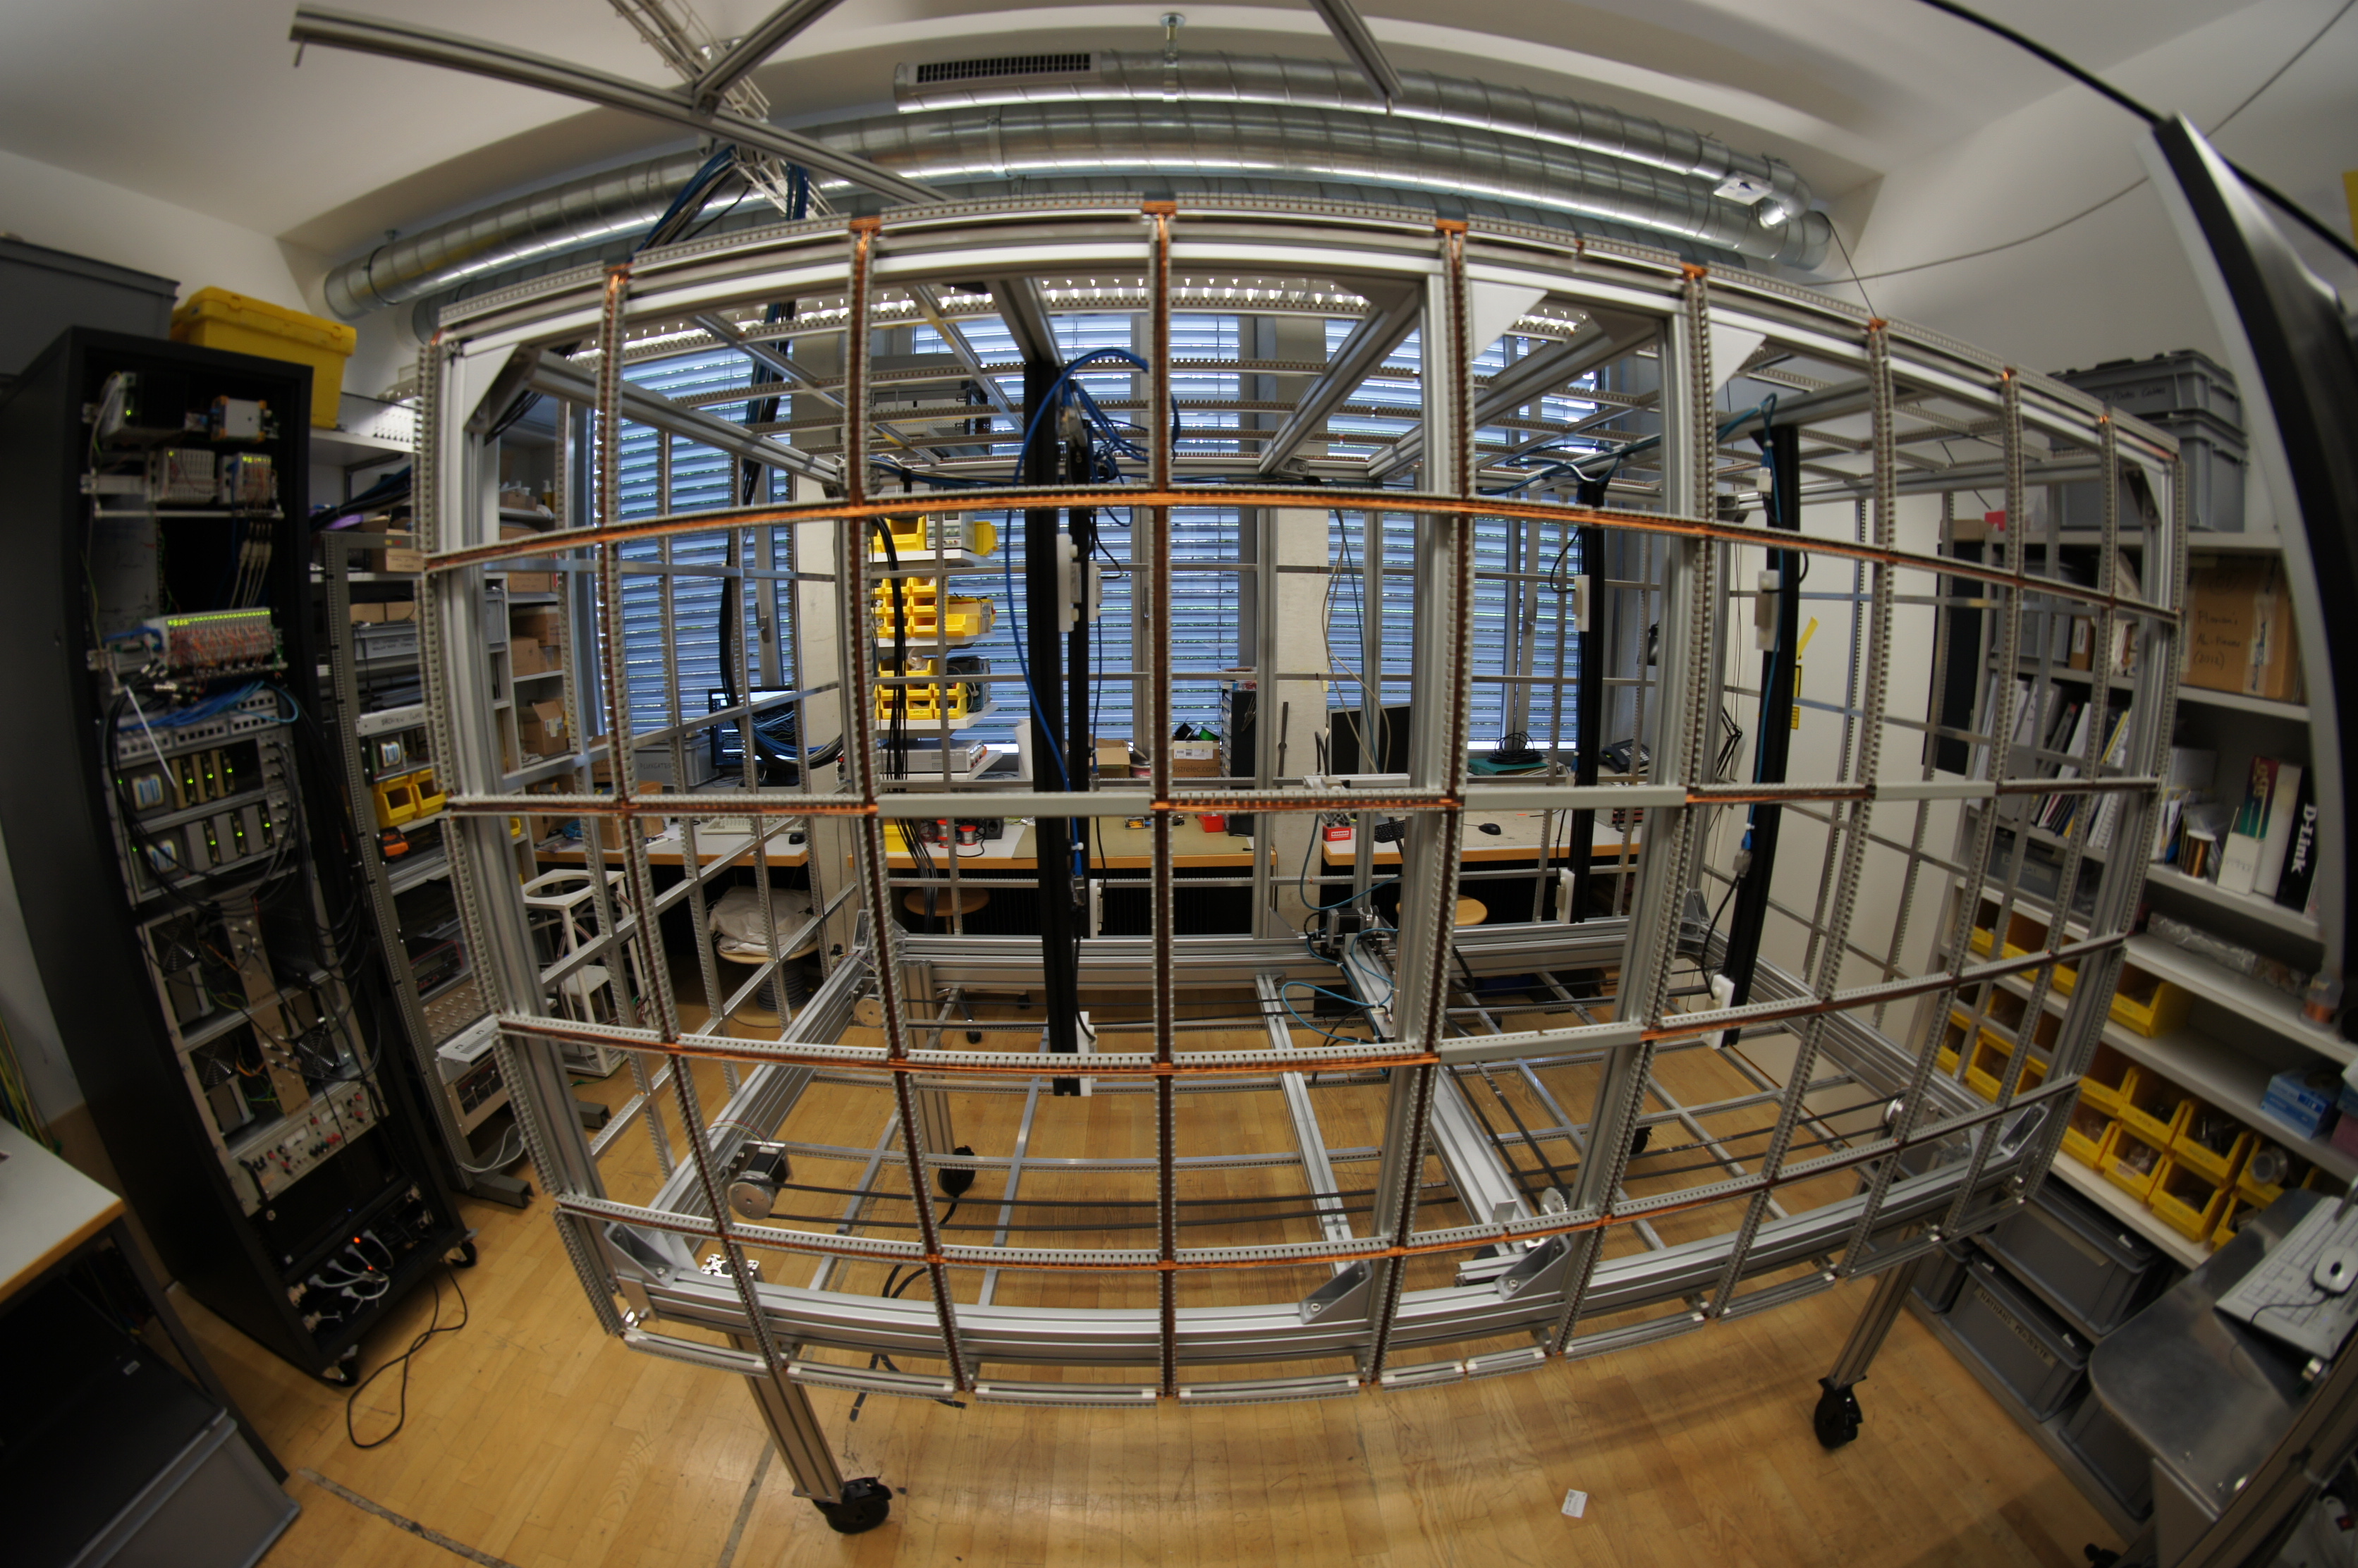
\includegraphics[width=0.75\linewidth]{gfx/prototype/DSC03472.JPG}
  \caption{The active magnetic shield in the laboratory at ETH Zürich. In the open cable channels the copper wires making up coils can be seen. The cable channels are held by an aluminum structure. On the left-hand side the control cabinet of the system is visible.}\label{fig:prototype_photo}
\end{sidewaysfigure}

\begin{figure}
  \centering
  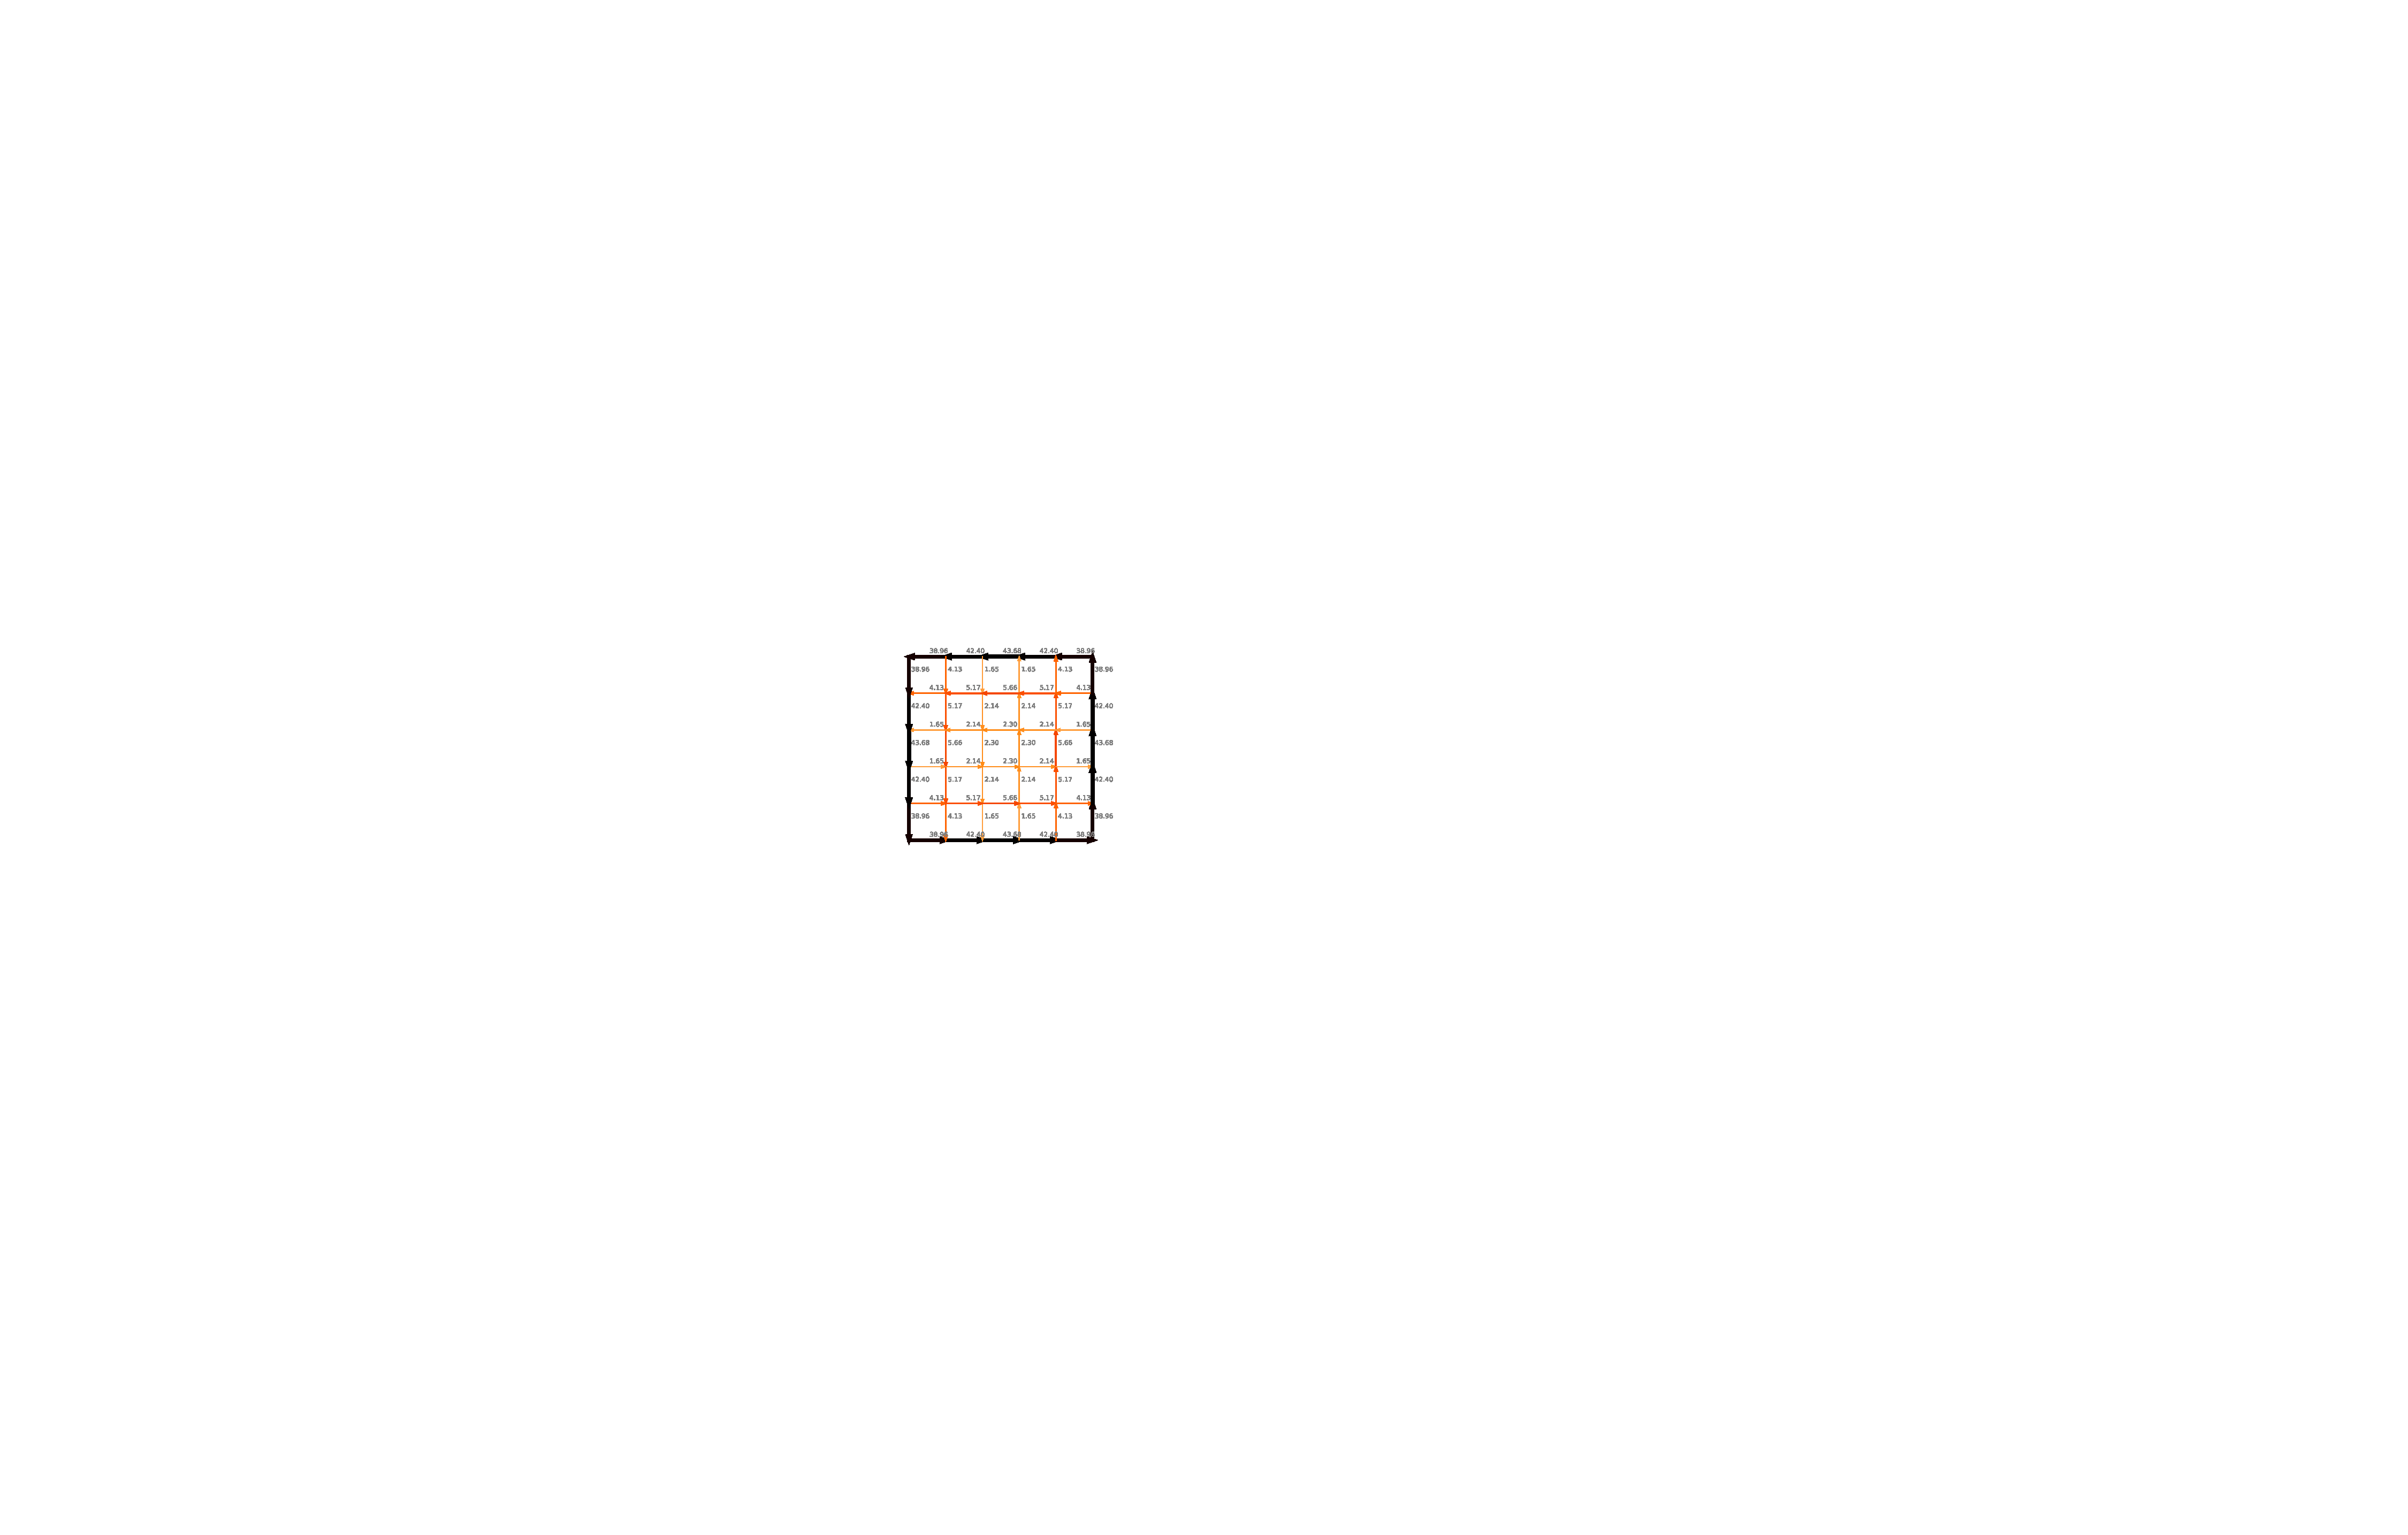
\includegraphics[height=0.3\linewidth]{gfx/prototype/coil_design_y_100uT_1.pdf}
  \quad\quad
  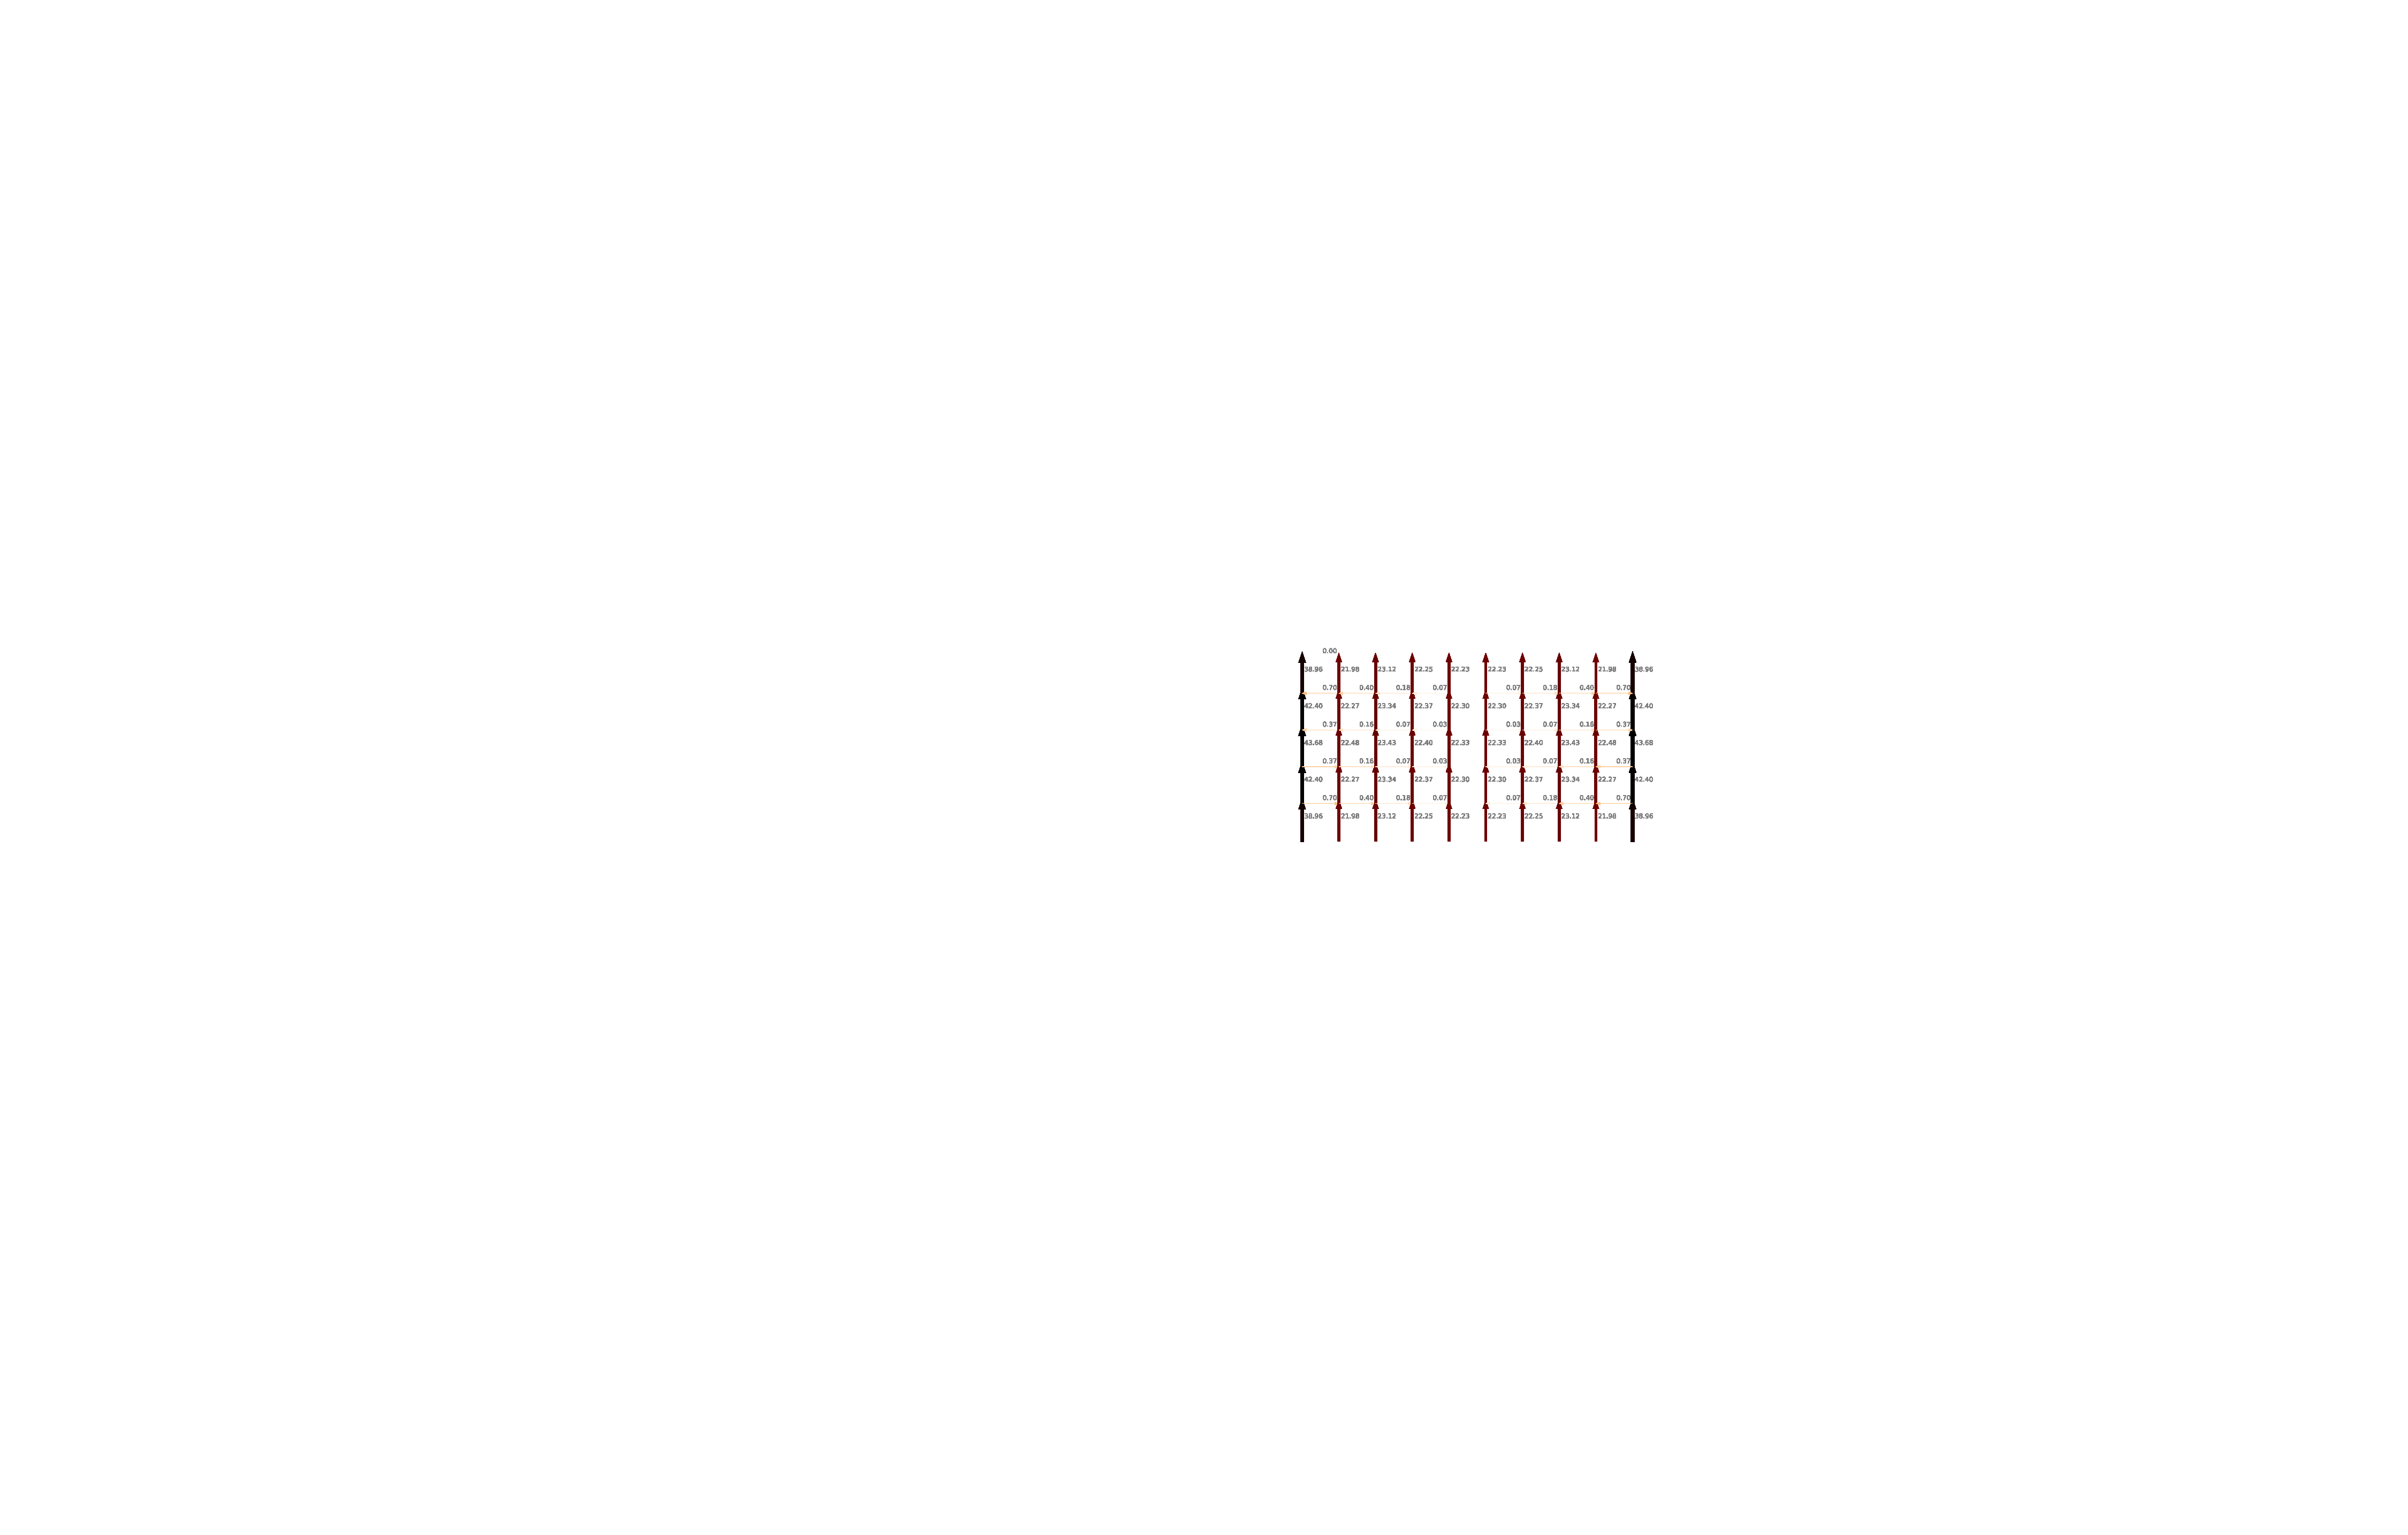
\includegraphics[height=0.3\linewidth]{gfx/prototype/coil_design_y_100uT_2.pdf}
  \caption{The optimal current net for the $y$-coil of ETH active magnetic shield. Both $5 \times 5$ faces ($y = \mathrm{const}$ planes) are identical and are depicted on the left-hand side. The rectangular faces are all identical, and are depicted on the right-hand side. For each segment the current per \SI{100}{\micro\tesla} of generated field is indicated upwards and to the right from its centre.}\label{fig:prototype_coil_y_currents}
\end{figure}

For the first version the system featured three coils for the homogeneous components of the magnetic field (the first three cartesian harmonics, Tab.\,\ref{tab:coils_cartesian_harmonics}).
The coils were mostly designed following the method described in Ch.\,\ref{ch:coil_design},
with the exception of the simplification algorithm, which was not ready at the time.
Instead, the simplification was carried out manually.
The fiducial volume was chosen to be a cuboid centred in the system, with each of its faces \SI{155}{\milli\meter} away from the surface of the coils.
The optimal current net for the $y$-coil (producing a homogeneous field in the $y$ direction) is depicted in Fig.\,\ref{fig:prototype_coil_y_currents} and its manual decomposition into loops in Fig.\,\ref{fig:prototype_coil_y_decomposition}.
The design promised a \SI{2}{\percent} homogeneity inside the fiducial volume.
The current net for $x$- and $z$-coils, identical to each other on symmetry grounds, is depicted in Fig.\,\ref{fig:prototype_coil_x_z_currents}.
Finally, the individual loops were discretised into \SI{10}{\ampere}, \SI{2}{\ampere} and \SI{0.2}{\ampere} per nominal \SI{100}{\micro\tesla}.
For example, the \SI{38.96}{\ampere} current, indicated in black in Fig.\,\ref{fig:prototype_coil_y_decomposition}, was realised as three windings of the \SI{10}{\ampere} wire, four of the \SI{2}{\ampere} wire and five of the \SI{0.2}{\ampere} wire.

\begin{figure}
  \centering
  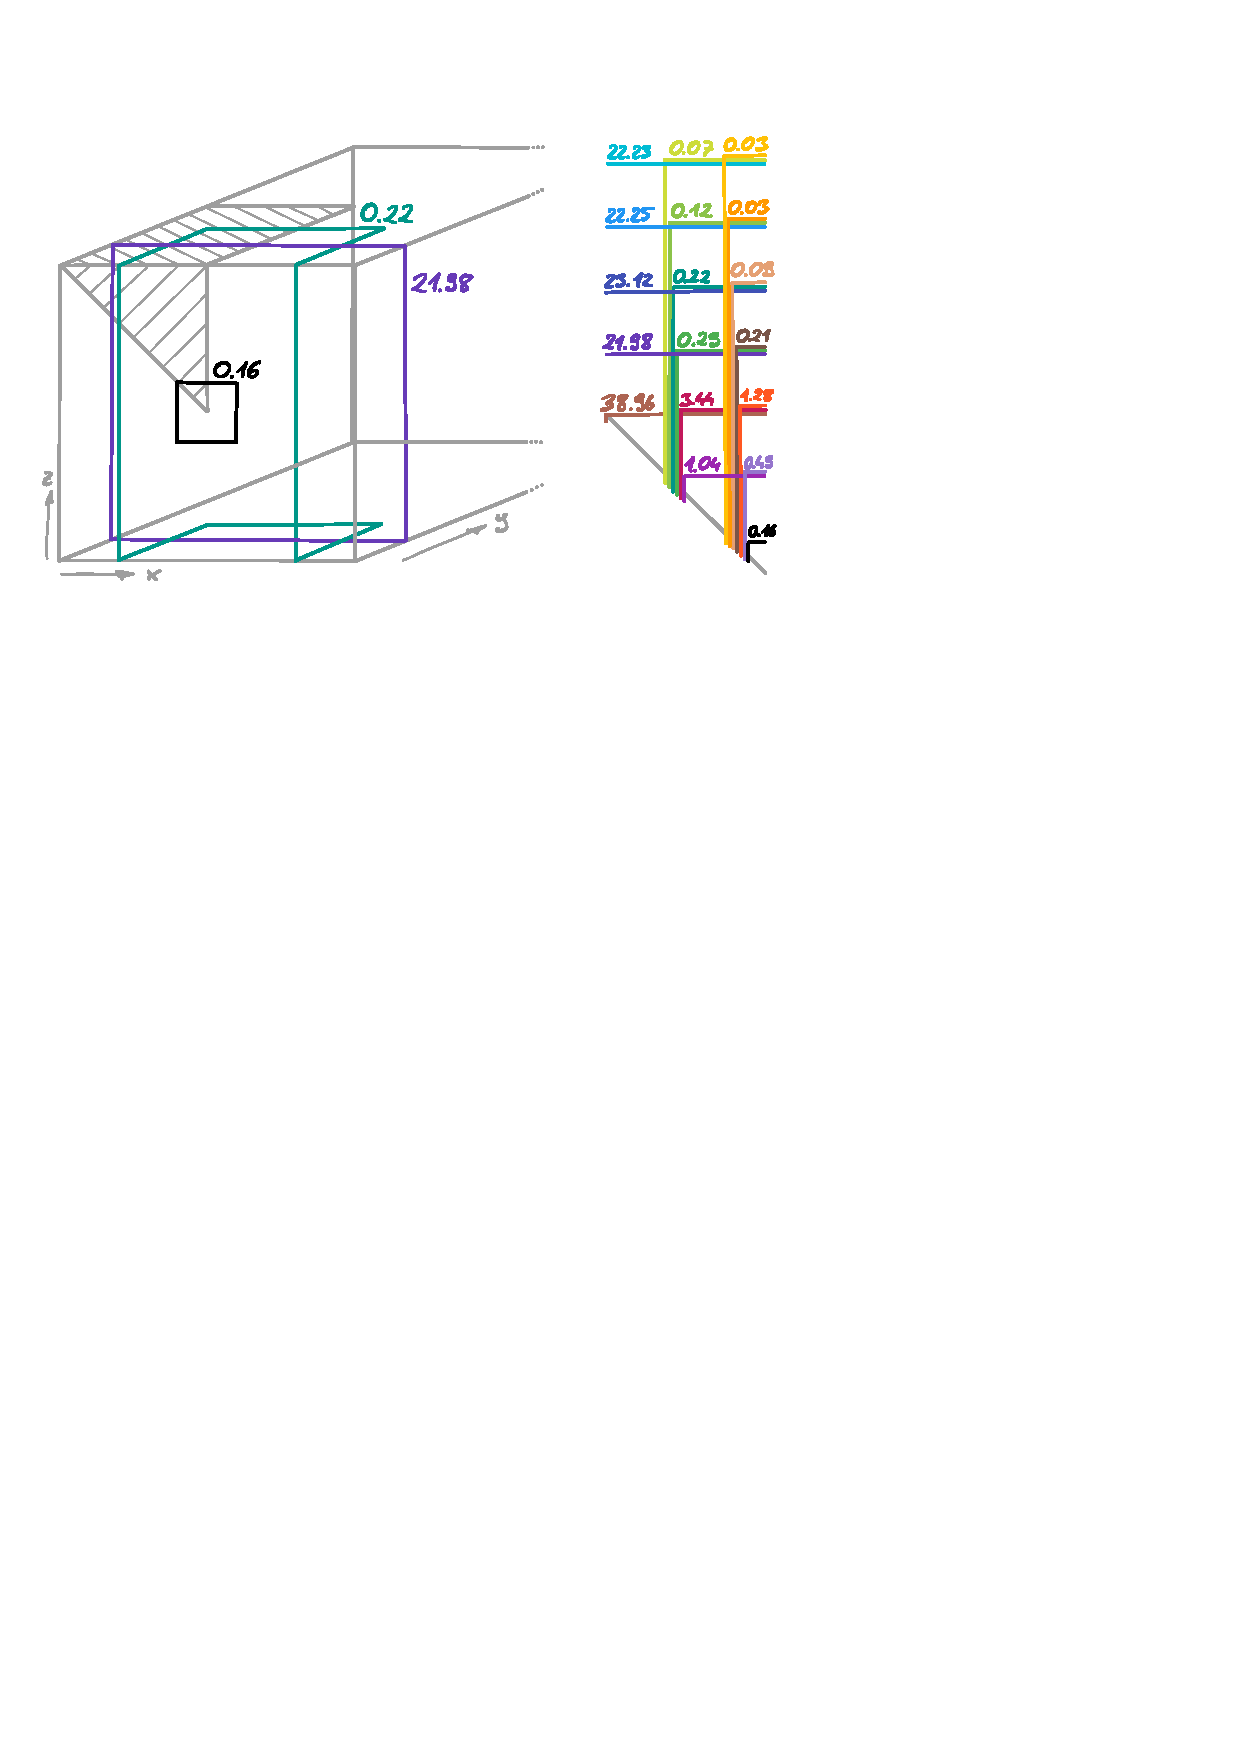
\includegraphics[width=0.9\linewidth]{gfx/prototype/coil_y_decomposition.pdf}
  \caption{The decomposition of the current net of the $y$-coil (Fig.\,\ref{fig:prototype_coil_y_currents}) into current loops. On the left-hand side only two loops are depicted in an isometric view. On the right-hand side a sixteenth part (dashed on the left) of the system is depicted, all others being identical on the grounds of symmetry. Each loop is indicated with a different colour. The currents are given per \SI{50}{\micro\tesla} of generated field.}\label{fig:prototype_coil_y_decomposition}
\end{figure}

\begin{figure}
  \centering
  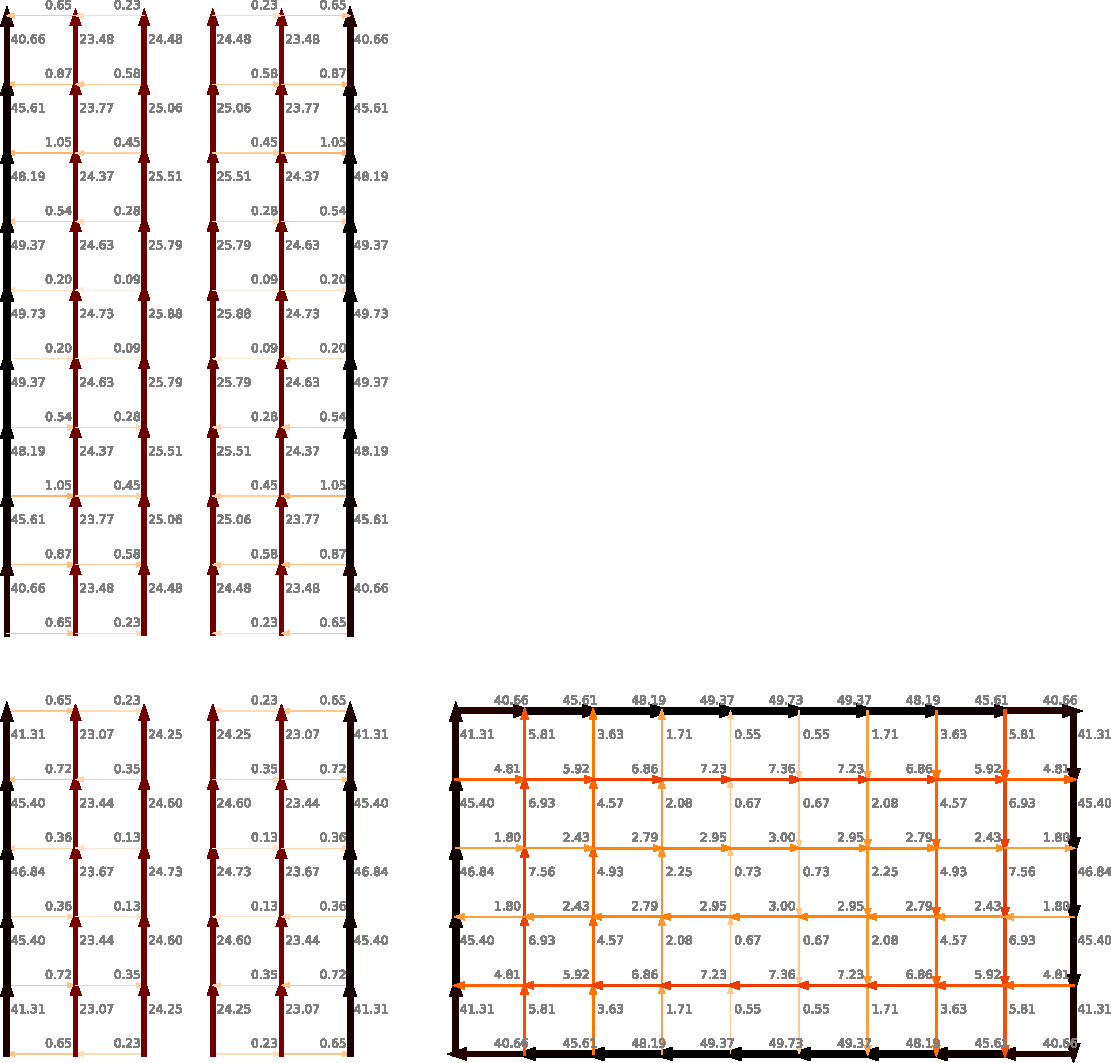
\includegraphics[width=0.9\linewidth]{gfx/prototype/coil_design_x_100uT.pdf}
  \caption{The optimal current net for the $x$ and $z$-coils of ETH active magnetic shield. Both $5 \times 5$ faces ($y = \mathrm{const.}$ planes) are identical, and are depicted in the lower-left corner. The rectangular faces perpendicular to the field are depicted to the right, and the ones parallel to it on top. For each segment the current per \SI{100}{\micro\tesla} of generated field is indicated upwards and to the right from its centre.}\label{fig:prototype_coil_x_z_currents}
\end{figure}

\begin{figure}
  \centering
  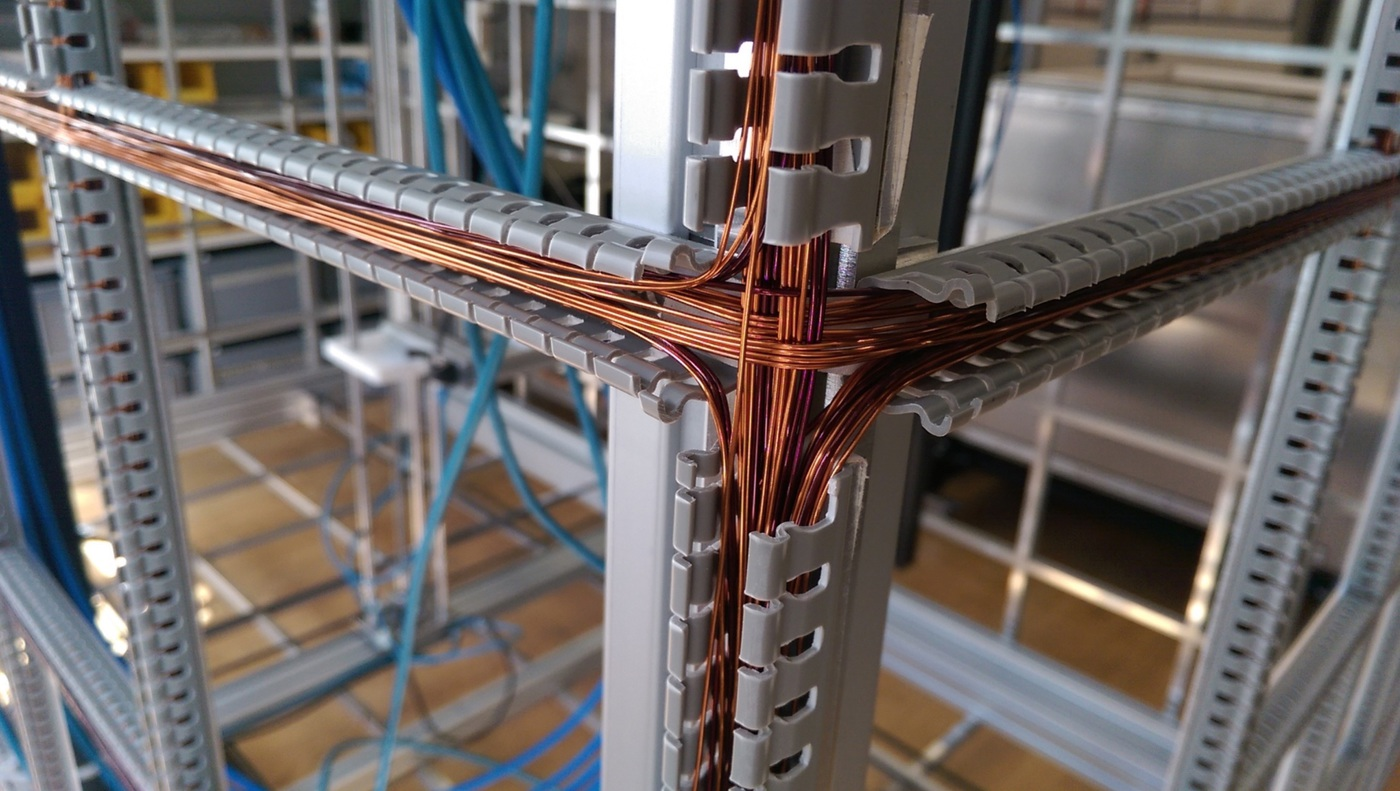
\includegraphics[width=0.9\linewidth]{gfx/prototype/wires_close_up.jpg}
  \caption{A close-up of the wires in the cable channels. Here all three coils for generating the homogeneous fields ($x$, $y$ and $z$) were laid.}\label{fig:prototype_coil_wire_close-up}
\end{figure}

\marginpar{The wire diameter was \SI[detect-all = true]{1}{\milli\meter} for the \num[detect-all = true]{10} and \SI[detect-all = true]{2}{\ampere} wires, and \SI[detect-all = true]{0.8}{\milli\meter} for the \SI[detect-all = true]{0.2}{\ampere} one. The wires were prolonged when needed.}
Enameled wire was laid in the cable channels according to the discretised design.
For one current component of a coil, e.g.\ \SI[detect-all = true]{10}{\ampere} in the $x$-coil, a single long piece of wire was laid, making up all the windings of all loops.
For the three coils, each with three components, nine long wires were laid in total.
A close-up of the wires in the cable channels, for all three coils, is shown in Fig.\,\ref{fig:prototype_coil_wire_close-up}.




\section{Mapping}
\label{sec:prototype_mapping}
The coils were mapped in order to verify that they produced a field of the required homogeneity.
To that purpose a robot was built: a fluxgate on an xyz-table, controlled with stepper motors.
The robot, called a \emph{mapper}, is pictured in Fig.\,\ref{fig:prototype_photo_inside}.

\begin{sidewaysfigure}
  \centering
  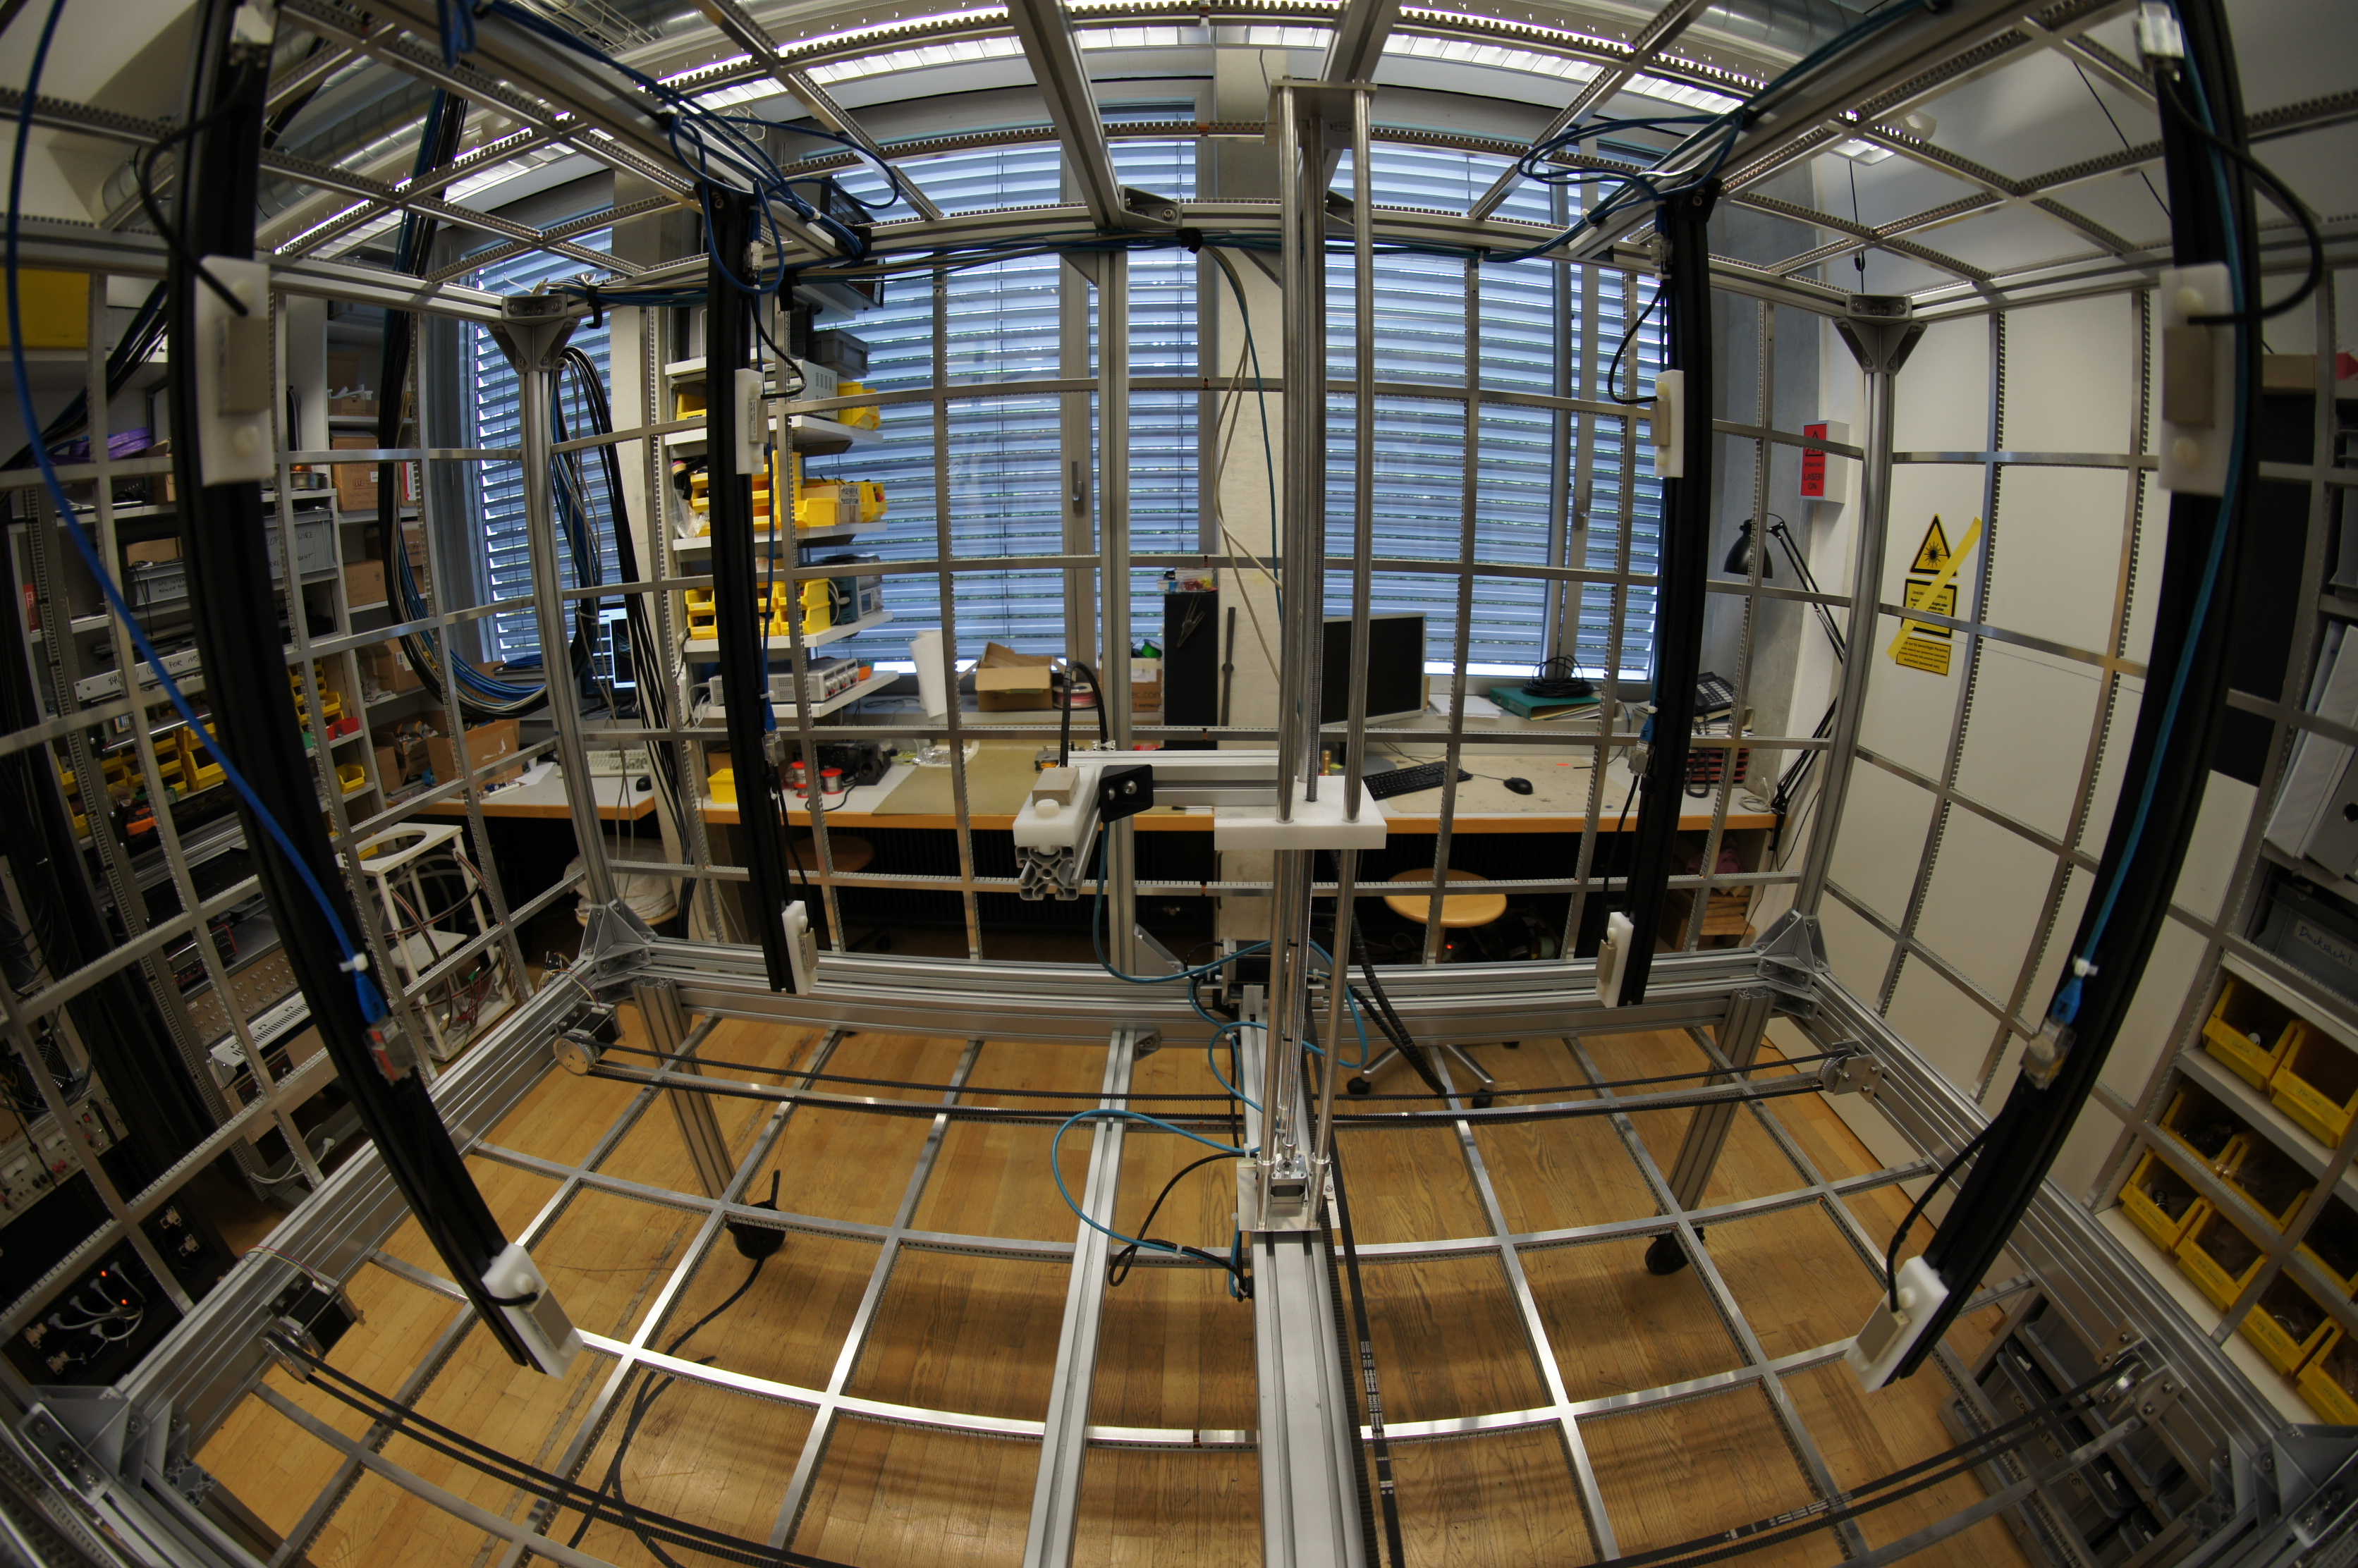
\includegraphics[width=0.75\linewidth]{gfx/prototype/DSC03476.JPG}
  \caption{The inside of the active magnetic shield. In the centre the mapping robot (\emph{mapper}) is visible, with a fluxgate magnetic field sensor mounted to a mobile platform. Mounted on black, vertical beams there are eight fluxgates for the active feedback.}\label{fig:prototype_photo_inside}
\end{sidewaysfigure}

A beam seen in the middle-bottom of Fig.\,\ref{fig:prototype_photo_inside} could move along the $y$ direction (left-right in the figure), pulled by two timing belts.
The belts were wound around pulleys attached to stepper motors, visible to the left.
Along the beam ($x$ direction) a cart was moved using the same method.
On the cart three vertical rods were attached with a plastic (POM) platform tightly threaded on them.
On the platform was a fluxgate magnetic field sensor.
\marginpar{In a fluxgate a ferromagnetic core is periodically driven into saturation. When it is not saturated, it is highly permeable and sucks the external magnetic flux in. When saturated, this does not occur. A pickup coil detects the changes in the external flux as it is alternately sucked in and out of the core.}
Through the centre of the platform was an aluminum threaded rod, passing through a mating threaded hole.
The rod was mounted to a stepper motor on the cart.
As the motor spun the threaded rod the platform moved vertically along the $z$ direction.

A simple map consists of moving the fluxgate along one linear direction only.
A map of the $y$-coil along the $y$ direction, in the middle of $x$ and $z$, is shown at the top of Fig.\,\ref{fig:prototype_linear_map}.
Only the $y$-component of the magnetic field is plotted. The coil was set to produce \SI{50}{\micro\tesla}.
The background field was also mapped and it has been subtracted in the map. The field remained in a $\SI{\pm 0.2}{\micro\tesla}$ range around the average value.
In the lower plot of Fig.\,\ref{fig:prototype_linear_map} the maps using just the \SI{10}{\ampere} component coil,
and \SI{10}{\ampere} and \SI{2}{\ampere} coils are shown (for \SI{50}{\micro\tesla} the currents were \SI{5}{\ampere}, \SI{1}{\ampere} and \SI{0.1}{\ampere}).
It is interesting to note how much of the field is produced by each of the components.
In the middle region the \SI{5}{\ampere}, \SI{1}{\ampere} and \SI{0.1}{\ampere} components produced \SI{86}{\percent}, \SI{11}{\percent} and \SI{3}{\percent} of the \SI{50}{\micro\tesla} field, respectively. At the edge the shares change to \SI{70}{\percent}, \SI{16}{\percent} and \SI{14}{\percent}.

\begin{figure}
  \centering
  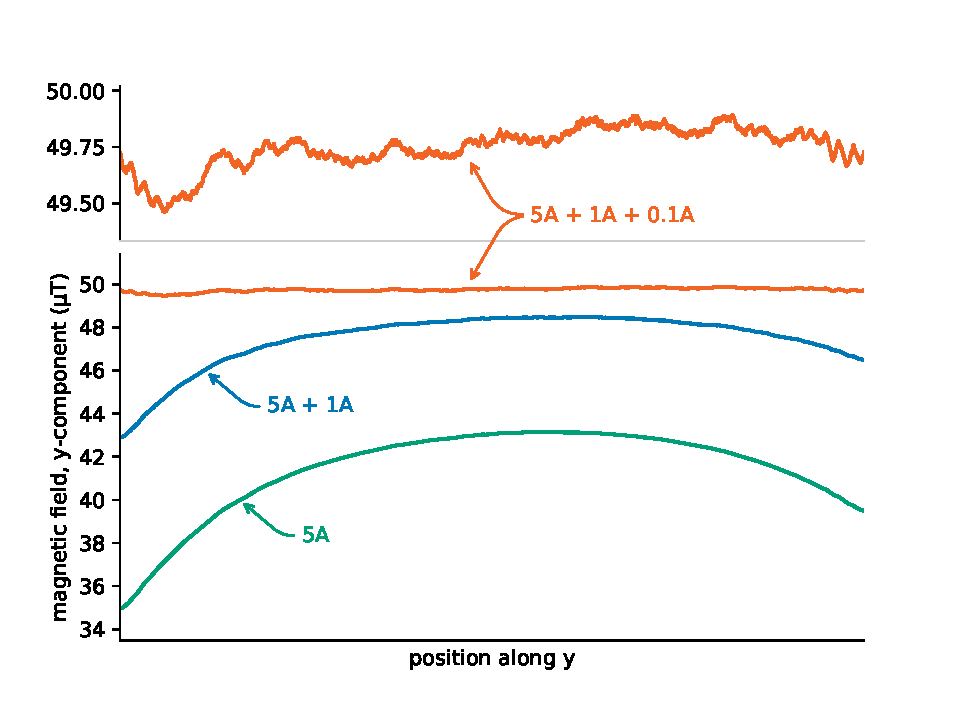
\includegraphics[width=0.9\linewidth]{gfx/prototype/y_scan_all_double.pdf}
  \caption{Linear map of the homogeneous field $y$-coil. The map is along the $y$-direction, in the middle of $x$ and $z$. The $y$-component of the magnetic field is plotted. The green curve depicts the field with only the \SI{5}{\ampere}/\SI{50}{\micro\tesla} wire, the blue with the additional \SI{1}{\ampere}/\SI{50}{\micro\tesla} wire, and the orange, also zoomed in at the very top, all three wires together.}\label{fig:prototype_linear_map}
\end{figure}

\begin{figure}
  \centering
  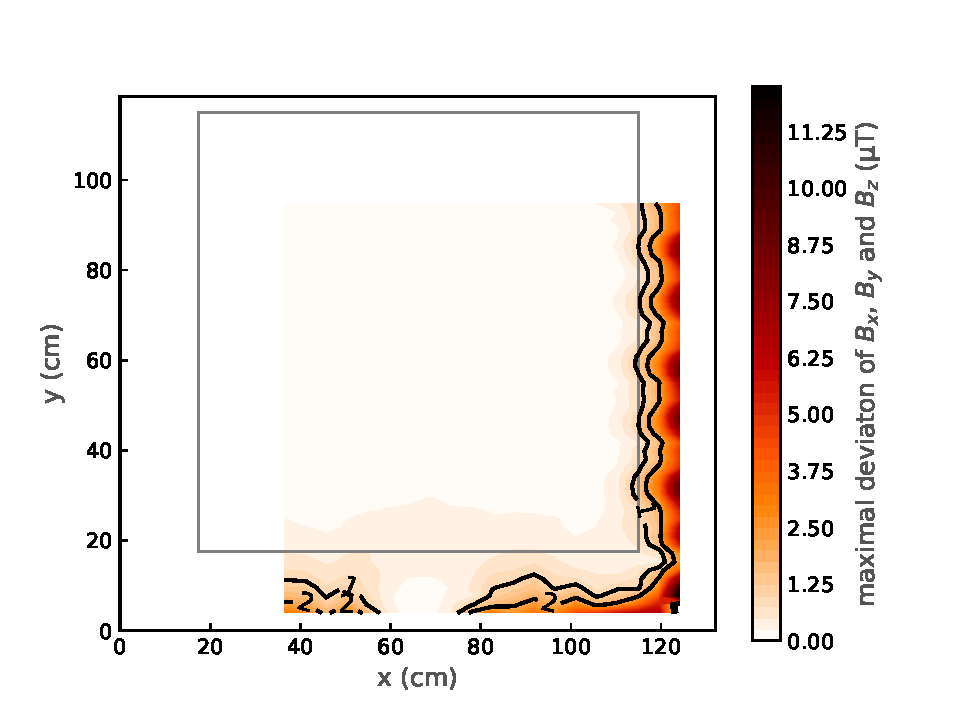
\includegraphics[width=\linewidth]{gfx/prototype/planar_map_Y_max_deviation.pdf}
  \caption{A horizontal map of the $y$-coil cut along the middle $xy$-plane. The maximum deviation among all three components of the magnetic field is plotted, i.e.\ in the area enclosed by the \SI{1}{\micro\tesla}~isocountour all components of the field are within \SI{1}{\micro\tesla} from the nominal field (zero for $x$ and $z$, \SI{50}{\micro\tesla} for $y$). Only part of the coil was mapped. The border of the plot corresponds to planes where the coil wires are located. The border of the fiducial volume is marked with grey lines.}\label{fig:prototype_plane_map}
\end{figure}

Another type of field map was a planar one.
A horizontal map in the middle $xy$-plane, of the $y$-coil is presented in Fig.\,\ref{fig:prototype_plane_map}.
The plot shows the maximum deviation among all three components of the magnetic field, i.e.\ in the area enclosed by the \SI{1}{\micro\tesla}~isocountour, all components of the field are within \SI{1}{\micro\tesla} from the reference field.
The reference field would ideally be zero for $x$ and $z$, and \SI{50}{\micro\tesla} for $y$.
In reality the sensor's axis were not perfectly aligned with those of the system,
causing the $x$ and $z$ components to be non-zero and the $y$ one to be smaller.
The reference field was set as the average field in the area of the highest homogeneity in the middle of the map.
Within the fiducial volume the field deviated by no more than \SI{2}{\percent} or \SI{1}{\micro\tesla} for a \SI{50}{\micro\tesla} field, as expected.
Maps of the other coils gave similar results.
%\mnote{Need to be clear about the specification---it wasn't supposed to be 2\% EVERYWHERE! Maybe bring forward the specification plot that decided on the grid size?}




\section{Control System}
In this section the hardware stack used to measure and control the magnetic fields is described.
% Before proceeding to discuss the active stabilisation system, we devote a section to the hardware. These are technical details, but for the more tech-savvy of the readers having the hardware setting given first may ease following the discussion.
In an active magnetic shield a change in the magnetic field is detected with an array of sensors, and an appropriate response is calculated.
The response is then applied by changing the currents in the coils.
The feedback loop is closed when the sensors detect the change in the field caused by the coils.

In the system at ETH the field was measured with eight fluxgates (visible in Fig.\,\ref{fig:prototype_photo_inside}).
They were mounted in a way to make up corners of a cube of approximately \SI{90}{\centi\meter} side length.
The sensors were Stefan Mayer Instruments FLC3--70 three-axis fluxgates, $\SI{\pm 200}{\micro\tesla}$ range, \SI{1}{\kilo\hertz} bandwidth, $\pm \SI{1}{\percent} \pm \SI{0.5}{\micro\tesla}$ accuracy.
They were powered with an in-house built $\SI{\pm 5}{\volt}$ power supply.
The outputs of the fluxgates were $\SI{\pm 5}{\volt}$ signals proportional to the magnetic field.
The analogue signals were directly digitised with Beckhoff EL3602 24-bit differential analogue-to-digital converters (ADCs).
The digital information was collected in software running on a PC.

\marginpar{The main julia program published the data on a \texttt{ZMQ} \texttt{PUB} socket. The data were stored with a separate \texttt{julia} program, collecting the data on a \texttt{ZMQ} \texttt{SUB} socket. Similarly, the plotting program was separate, written in \texttt{Python}.}
The software stack running under OpenSUSE Linux consisted of a low-level Ethercat driver~\cite{etherlabcode}, on top of which a custom program written in \texttt{julia}~\cite{julia} was running.
This setup was optimised for high flexibility and close-to-zero turnaround time during the development.
In particular, it was possible to develop the software interactively \emph{while} the system was running.
The main task of the program was to continuously evaluate the optimal response for the measured magnetic field changes.
The response, being the new currents to be applied to the coils, was sent to the digital-to-analogue converters (DACs). The data were recorded and plotted on-line.

The DACs were 16-bit Beckhoff EL4134.
The signals were fed to an array of four-quadrant SERVOWATT amplifiers, configured to regulate the output current with a $\SI{\pm 10}{\volt}$ input.
For each coil there were three stages: DCP260/30A configured with a $\SI{\pm 10}{\ampere}$ output, DCE50/30A with $\SI{\pm 2}{\ampere}$ and DCE10/30A with $\SI{\pm 0.4}{\ampere}$.
The currents were then directly fed into the coils.

\begin{SCfigure}
  \centering
  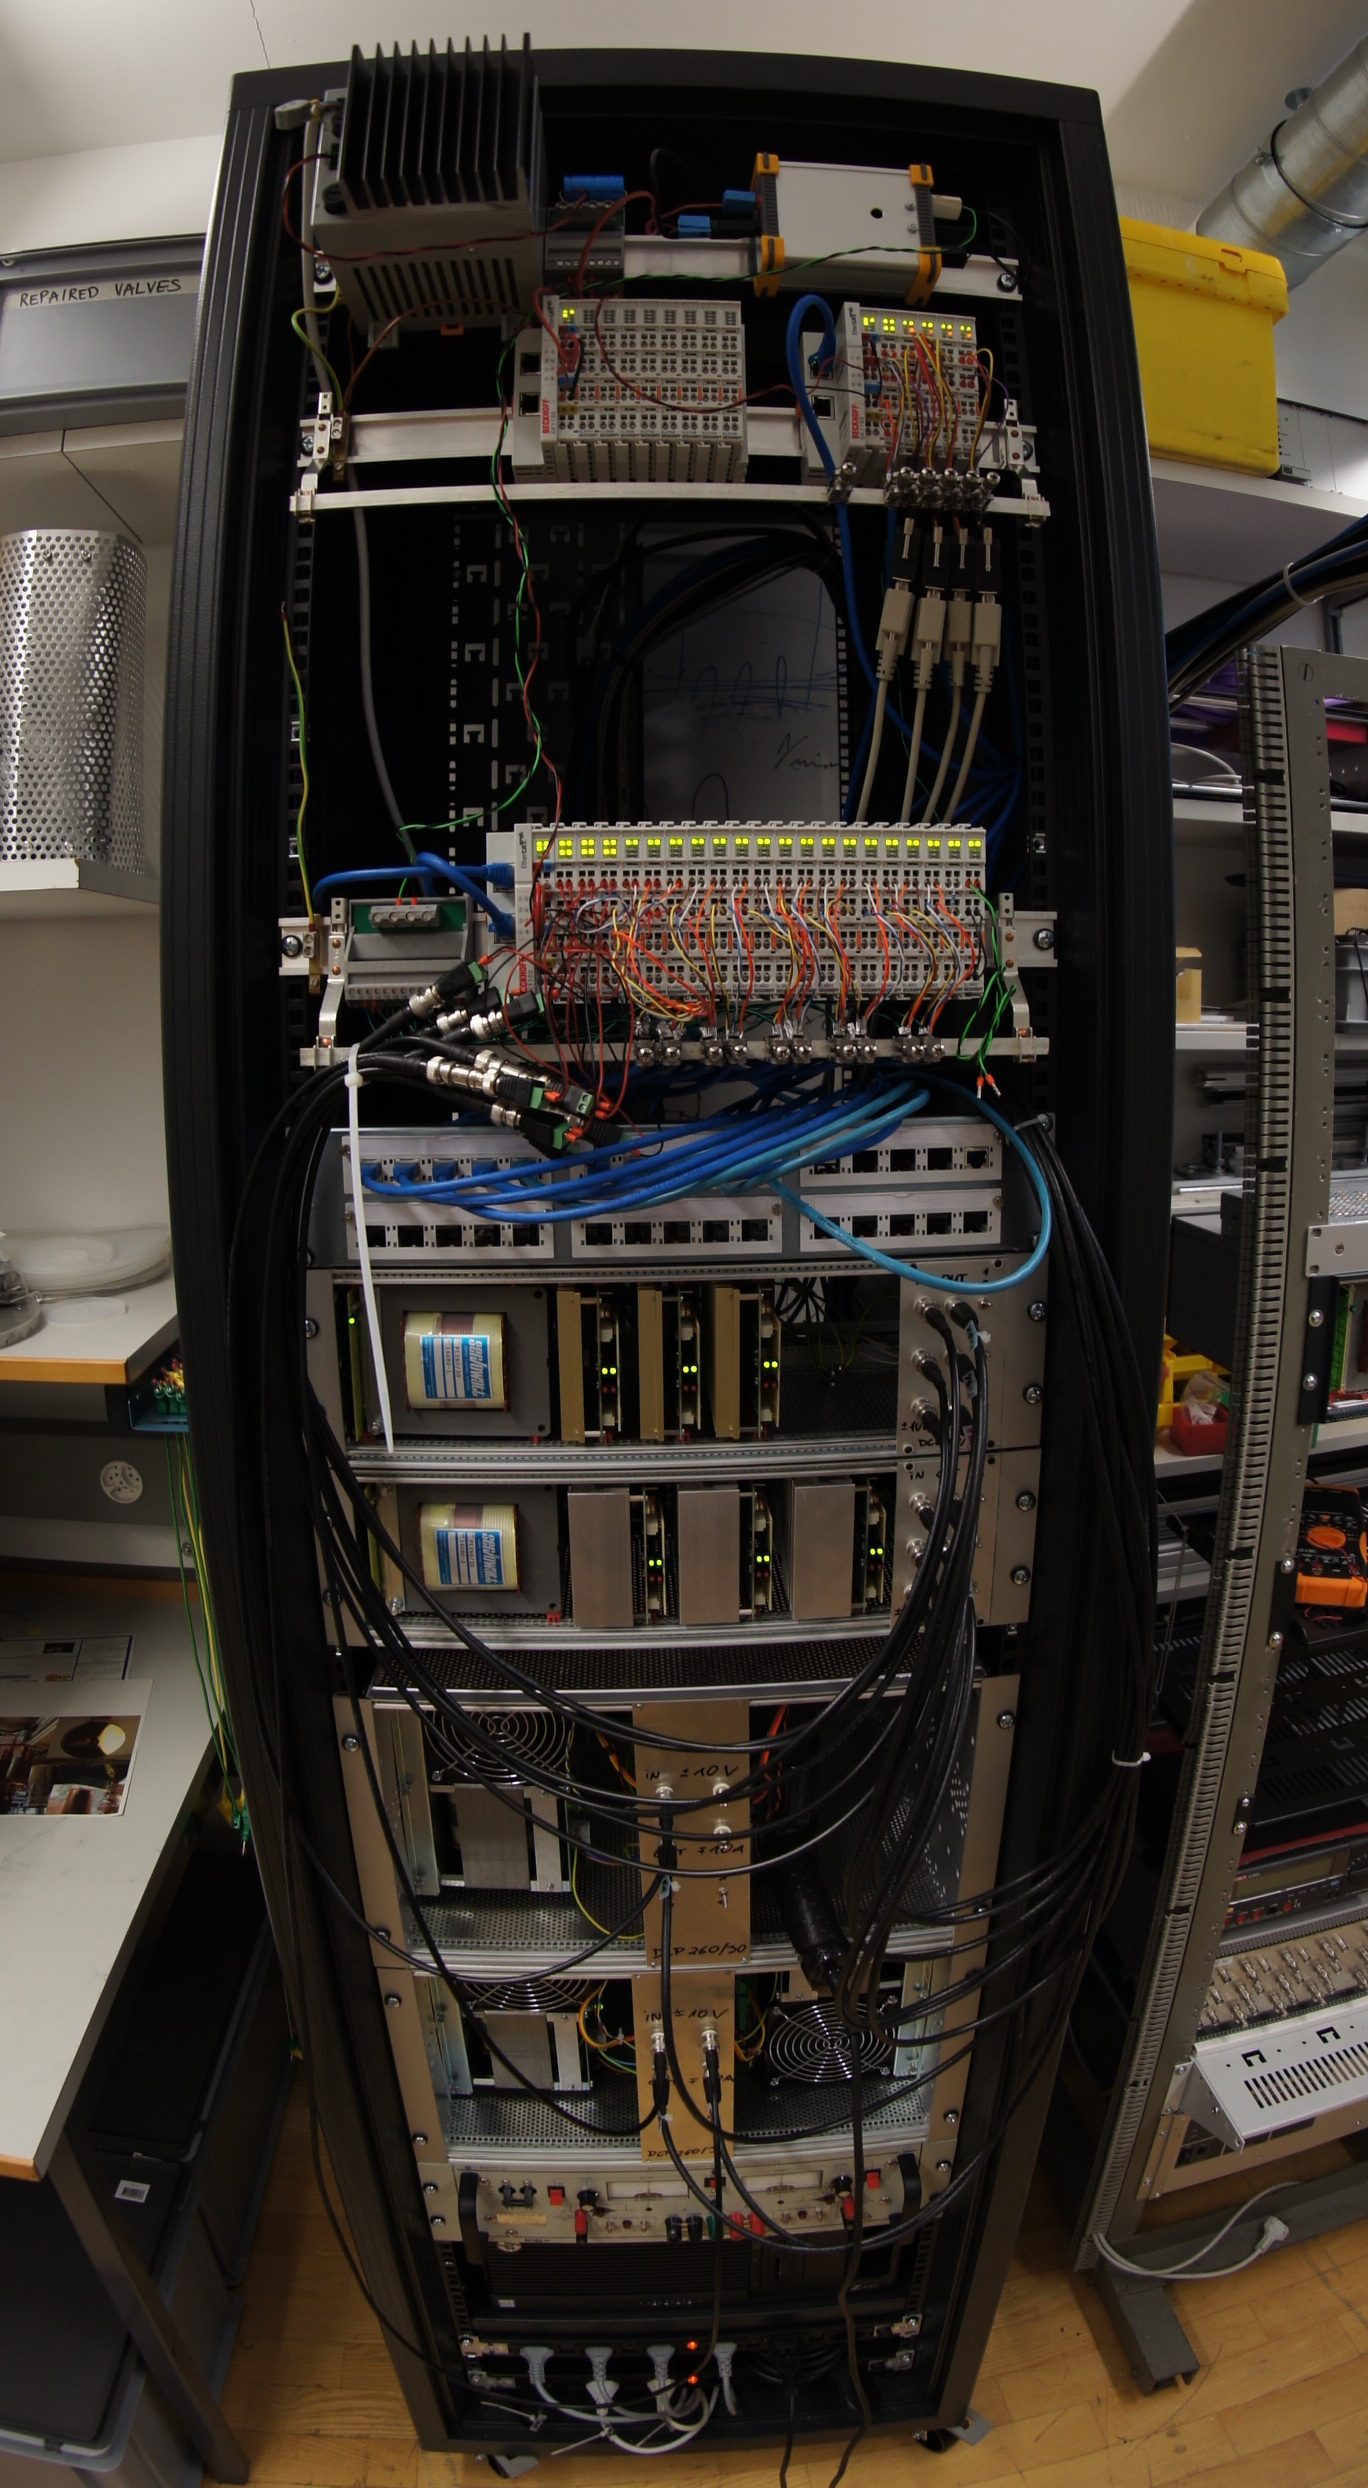
\includegraphics[width=0.6\linewidth]{gfx/prototype/DSC03477_cropped.jpeg}
  \caption{The 19-inch cabinet hosting the electronics for the active magnetic field shield. From top: a \SI{24}{V} power supply for the Beckhoff EtherCAT clamps and in-house--built $\SI{\pm 5}{\volt}$ power supply for the fluxgates; spare EtherCAT clamps and control system for the mapper; a large array of EtherCAT DACs and ADCs for the active stabilisation system; breakout panel for the fluxgate cables (RJ-45 plugs); subrack with $\SI{\pm 0.4}{\ampere}$ amplifiers; subrack with $\SI{\pm 2}{\ampere}$ amplifiers; two subracks with $\SI{\pm 10}{\ampere}$ amplifiers; a general-purpose Kepco $\SI{\pm 20}{\volt}$ $\SI{\pm 20}{\ampere}$ four-quadrant amplifier; the PC.}\label{fig:prototype_photo_daq}
\end{SCfigure}

The hardware was hosted in a 19-inch cabinet, pictured in Fig.\,\ref{fig:prototype_photo_daq}.
A detailed list of the components can be found in the figure's caption.
All these components were used for the active magnetic field shielding.




\section{The feedback matrix}
The system was based on a feedback matrix (Ch.\,\ref{ch:nedm_sfc}).
The magnetic field measured by each of the 24 sensors is linear with the currents in the three coils.
All readouts, gathered in a vector $\mathbb{B}$ (dimension~24) can be written as a linear combination of the currents in the coils $\mathbb{I}$ (dimension~3):
\marginpar{We use the symbol $\mathbb{B}$ for the values measured by the sensors to distinguish it from $\mathbf{B}$, which is used to denote the magnetic field in the whole space.}
\begin{equation}
  \label{eq:SFC_matrix_model}
  \mathbb{B} = M \mathbb{I} + \mathbb{B}_0 \ ,
\end{equation}
where $\mathbb{B}_0$ is the free offset.
The matrix of proportionality constants $M$, dimension $24 \times 3$, is the central element of the active shield.

Let us recall the discussion of the PSI system's matrix in Sec.\,\ref{fig:nEDM_SFC_matrix}.
There it was pointed out that its high condition number, and the need for regularisation, can be attributed to the geometry of the system.
In particular, some linear combinations of the coils created high-order fields which, despite high currents, had little influence on the sensors' readout.
% The matrix of the PSI system and its properties were thoroughly discussed in Sec.\,\ref{fig:nEDM_SFC_matrix}.
% There is a fundamental difference between the matrix of the PSI's system and the one of the next generation's one.
PSI SFC matrix was not known a priori.
The system was constructed and the matrix was measured as the system's property. \note{Previous unclear, reformulate}
% This could be considered as the reason that the matrix was ill-conditioned and the system required regularisation and PI control to be stable.
Conversely, the new system already takes the matrix into account at the design phase.
The coils were designed to produce a magnetic field corresponding to the terms of the cartesian harmonic expansion of the field; 
ensuring that they are orthogonal to one another.
By design we expect the matrix to have the condition number equal to one.
Using the three coils it has been measured to be \num{1.064} for the homogeneous components, without a mu-metal shield inside.

% \note{Put a figure about the measurement of the matrix?}

The active magnetic shield constructed at ETH implemented a new way of measuring the matrix.
The procedure changed currents in all the coils simultaneously, shortening the duration of the procedure.
It could also measure in close-to-zero field conditions.
To measure the matrix, the space spanned by all the coils was considered.
In this case it was three-dimensional: the current in the $x$-coil, in the $y$-coil and in the $z$ one.
A point in this space corresponded to one configuration of the currents in the coils.
A set of points on an n-sphere in this space was picked and all currents were changed simultaneously, making their way from one point to another.
As the currents changed, the measurements of the sensors were recorded.
Then, for each $i$th readout channel (24 in total) a linear model was fitted to estimate the proportionality constants between the readout and the currents in the coils:
\begin{equation}
  \label{eq:SFC_matrix_linear_fits}
  B_i = B_i^0 + \sum_{j=x,y,z} M_{i,j} \, I_j \ ,
\end{equation}
where $B_i$ is the readout channel ($i$ going from 1 to 24), $I_j$ are the currents in the coils ($j$ going over $x$, $y$ and $z$) and $M_{i,j}$ is the matrix of proportionality constants---the feedback matrix.
$B_i^0$ is the free offset vector---the background field.

\marginpar{It is possible to fit the linear model and estimate the uncertainty of the matrix elements \emph{while} measuring; the measurement can be stopped when the uncertainty drops below a threshold.}
If the system is perfectly linear it does not matter where in the current-space the n-sphere is located, nor how large it is (though larger ones give more precise estimates per point).
However, we expect non-linearities to appear in the presence of a $\mu$-metal shield inside the system.
In that case it is preferable to measure the matrix in the vicinity of the point where the system is later operated.
Motivated by this, the following procedure of the matrix measurement was employed:
First an n-sphere centred at n-zero and a radius of \SI{50}{\micro\tesla} was chosen.
Then the system walked over ten random points on the sphere, taking two seconds to pass from one to the next (\SI{20}{\second} in total).
This gave the first estimate of the matrix.
The next sphere was chosen to be centred around the zero field. This is the optimal, in the least-squares sense, solution of Eq.\,\ref{eq:SFC_matrix_model} with $\mathbb{B} = 0$:
\begin{equation}
  \label{eq:SFC_zero_field_requirement}
  \mathbb{I}_\text{zero-field} = - M^\dagger \, \mathbb{B}_0 \ ,
\end{equation}
where $\mathbb{B}_0$ is the free offset from Eq.\,\ref{eq:SFC_matrix_linear_fits}, and $M^\dagger$ is the Moore-Penrose pseudoinverse of the matrix $M$.
This gave the second estimate of the matrix.
Finally, the measurement was repeated with a sphere again centred at zero, but with a smaller radius of \SI{1}{\micro\tesla}.
% The procedure was developed for a system with mu-metal.
In the case of an air system, without a mu-metal shield inside, all consecutive estimates of the matrix were almost the same.
% \note{Hopefully I still do get to measure the matrix with the mu-metal cube inside. Then I will describe it here.}

\begin{figure}
  \centering
  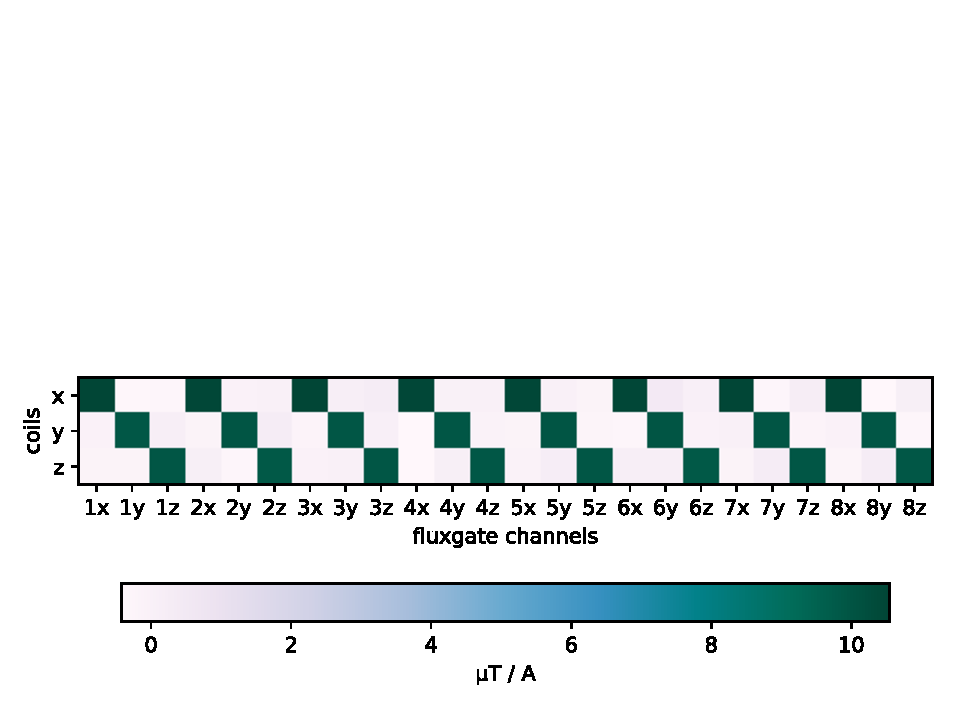
\includegraphics[width=.9\linewidth]{gfx/prototype/SFC_matrix_green.pdf}
  \caption{The measured feedback matrix of the active magnetic shielding system. The sensors were mounted $\approx\SI{20}{\centi\meter}$ away from the coil surface. The values are microteslas of field per \SI{1}{\ampere} in the strongest coil (\SI{0.2}{\ampere} and \SI{0.02}{\ampere} in the other two).}\label{fig:prototype_feedback_matrix}
\end{figure}

The matrix measured with the sensors $\approx\SI{20}{\centi\meter}$ away from the coil surface is presented in Fig.\,\ref{fig:prototype_feedback_matrix}.
The differences between the non-zero elements of different fluxgates are under 1\%, as expected from the design and the field map (Fig.\,\ref{fig:prototype_plane_map}).
The condition number of the matrix is \num{1.064}.
% A typical measured matrix is\ldots Estimate the field inhomogeneity right away from it! Give two at two distances, maybe? The one I looked at has around 0.5\% std homogeneity at the sensors' positions.

% Then continue to analyse the matrix. Discuss the SVD decomposition and its singular values. Or is it the right place to do it here?



\section{The feedback algorithm}
The feedback was based on calculating the optimal solution of Eq.\,\ref{eq:SFC_matrix_model} in each step.
In the $n$th iteration (the iteration index marked on top) the equation is
\begin{equation}
  \mathbb{B}^n = M \mathbb{I}^n + \mathbb{B}_0^n \ .
\end{equation}
In the next iteration the field equal to the target field is sought
\begin{equation}
  \mathbb{B}^{n+1} \overset{!}{=} \mathbb{B}_\text{target} \ .
\end{equation}
We allow $\mathbb{B}_\text{target}$ to be any field.
This leads to the following requirement for the next currents:
\begin{align}
  \mathbb{I}^{n+1} &=
    M^\dagger \left( \mathbb{B}_\text{target} - \mathbb{B}_0^{n+1} \right) \nonumber \\
    &\approx M^\dagger \left( \mathbb{B}_\text{target} - \mathbb{B}_0^{n} \right) \nonumber \\
    &= M^\dagger \left( \mathbb{B}_\text{target} - \mathbb{B}^n + M \mathbb{I}^n \right) \nonumber \\
    &= M^\dagger \left( \mathbb{B}_\text{target} - \mathbb{B}^n \right) + M^\dagger M \mathbb{I}^n \nonumber \\
    &= M^\dagger \left( \mathbb{B}_\text{target} - \mathbb{B}^n \right) + \mathbb{I}^n \ . \label{eq:current_update}
\end{align}
By defining $\Delta\mathbb{I}^n := \mathbb{I}^{n+1} - \mathbb{I}^{n}$ and $\Delta\mathbb{B}^n = \mathbb{B}^n - \mathbb{B}_\text{target}$ we obtain the intuitive rule for the current update
\begin{equation}
  \Delta\mathbb{I}^n = - M^\dagger \Delta\mathbb{B}^n \ .
\end{equation}
A careful reader may be alarmed by the approximation $\mathbb{B}_0^{n+1} \approx \mathbb{B}_0^{n}$ In Eq.\,\ref{eq:current_update}.
It is an unfortunate necessity, for the calculation needs to be performed just before the iteration $n+1$, when $\mathbb{B}_0^{n+1}$ is not yet known.
In other words, the correction needs to be delayed by at least one iteration.
This introduces lag, and motivates high feedback frequencies.

\begin{figure}
  \centering
  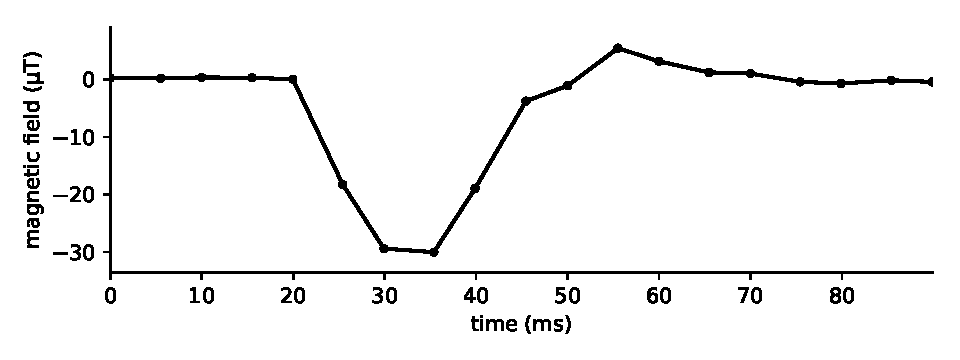
\includegraphics[width=.9\linewidth]{gfx/prototype/SFC_step_response.pdf}
  \caption{The reaction of the active magnetic field compensation to a step change in the magnetic field ($\approx \SI{30}{\micro\tesla}$ in \SI{5}{\milli\second}). The system was running at a rate of \SI{200}{\hertz}. Each dot marks one iteration.}\label{fig:prototype_step_response}
\end{figure}

In practice, the active shield had a delay of more than one iteration.
Although the system was operated at \SI{200}{\hertz}, the quickest turnaround was three cycles (\SI{15}{\milli\second}).
This was tested by applying a pulse on a DAC channel and observing the response on a directly connected ADC channel.
It appeared only in the third iteration after the pulse had been sent.
Knowing that the magnetic field information is delayed, it was crucial to delay the current information too, so Eq.\,\ref{eq:current_update} becomes:
\begin{equation}
  \mathbb{I}^{n+1} = M^\dagger \left( \mathbb{B}_\text{target} - \mathbb{B}^{n-2} \right) + \mathbb{I}^{n-2} \ .
\end{equation}
Without accounting for the delay the system would spontaneously destabilise.
In Fig.\,\ref{fig:prototype_step_response} a response of the system to a step-like change of the magnetic field is plotted.
Note how the system's reaction is delayed by three iterations.

% \note{A paragraph (or a margin note) comparing the feedback algorithm to the old one. Requires no parameters, any field may be the target field.}

% \note{Has been tested with the big system, but it did not outperform in terms of stability (do I have a plot to prove that?). Nick Schwegler's project report! I could just cite it here, it was inconclusive. But for sure I can say it.}




\section{Dynamic stabilisation}
\label{sec:dynamic_stabilisation}
The dynamic stabilisation was tested with a strong permanent magnetic dipole.
The dipole was built out of two extremely strong neodymium magnets (\SI{200}{\kilo\gram} force when attached to iron) connected together with a \SI{1}{\metre} long iron rod.
The dipole was moved several meters from the system causing a magnetic field disturbance.

% \mnote{Need to put the details of the geometry of the fluxgates here. Eight fluxgates on the corners of a cube of \ldots size.}

\begin{figure}
  \centering
  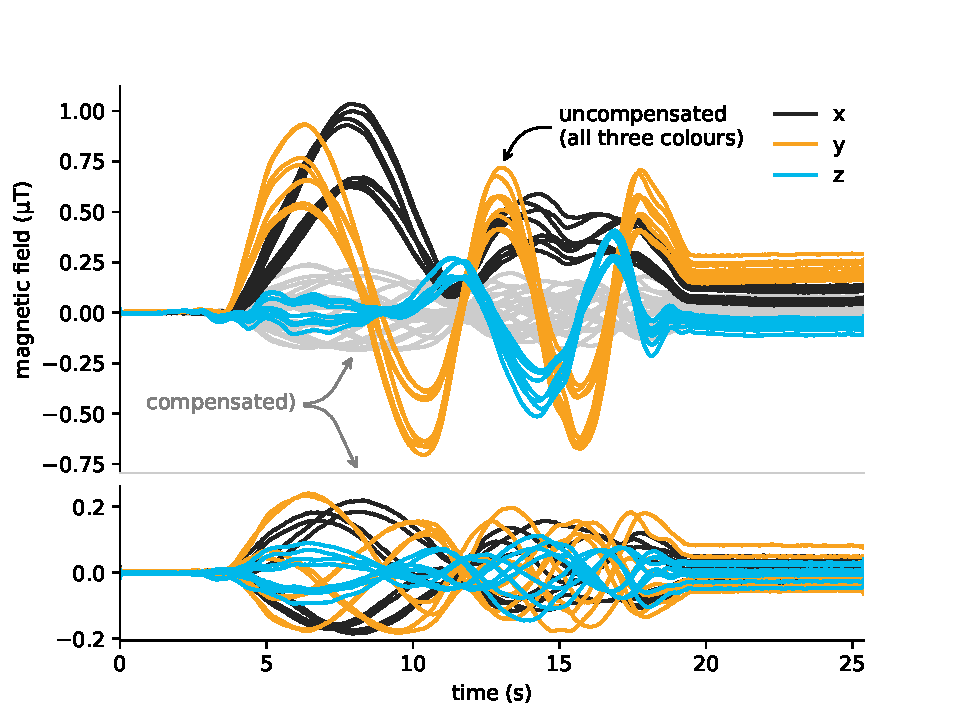
\includegraphics[width=\linewidth]{gfx/prototype/compensated_7_5m_double.pdf}
  \caption{Field variations caused by a rotating dipole \SI{7.5}{\meter} away.
  The upper part shows in colours corresponding to the spatial directions the uncompensated field $\mathbb{B}_0$ for all eight sensors, calculated according to Eq.\,\ref{eq:uncompensated_field}. Each line is one sensor. The compensated field $\mathbb{B}$ is depicted in grey in the upper part and is enlarged in the lower part of the plot in colour. The curves have been smoothed for clarity.}\label{fig:prototype_compensation_time}
\end{figure}

The resulting field compensation from the dipole being rotated \SI{7.5}{\meter} away from the system's centre are plotted in Fig.\,\ref{fig:prototype_compensation_time}. The upper part of the plot shows the field as it would be registered without compensation $\mathbb{B}_0$, calculated according to Eq.\,\ref{eq:SFC_matrix_model}:
\begin{equation}
  \label{eq:uncompensated_field}
  \mathbb{B}_0 = \mathbb{B} - \mathbb{M} \mathbb{I} \ .
\end{equation}
% The three colours correspond to the three spatial components ($x$, $y$, $z$). Each line is one sensor.
The measured field $\mathbb{B}$ is depicted in the bottom part.
The amplitude of the changes was reduced from around \SI{1.75}{\micro\tesla} to \SI{0.4}{\micro\tesla} (factor four).
Yet, the variation is not completely mitigated.

Looking at the orange lines in the upper part of Fig.\,\ref{fig:prototype_compensation_time}, each representing the readout of a different sensor in the $y$ direction.
The lines do not overlap, meaning that the field change was not homogeneous (which, of course, would be the same everywhere).
The coils of the system, being able to generate only homogeneous fields can only compensate the homogeneous part.
Graphically it may be explained in the following way: each of the coils coil can keep all lines in one of the colours (one spatial component) steady, but it cannot bring them closer together (homogenise the field).
This can be observed in the bottom part of Fig.\,\ref{fig:prototype_compensation_time}.
There lines are centred around zero, but their spread within one colour (spatial component) is not reduced.
In order to do that, coils producing higher-order fields would be required.
% After all, the active compensation can compensate only as much as it can.

\begin{figure}
  \centering
  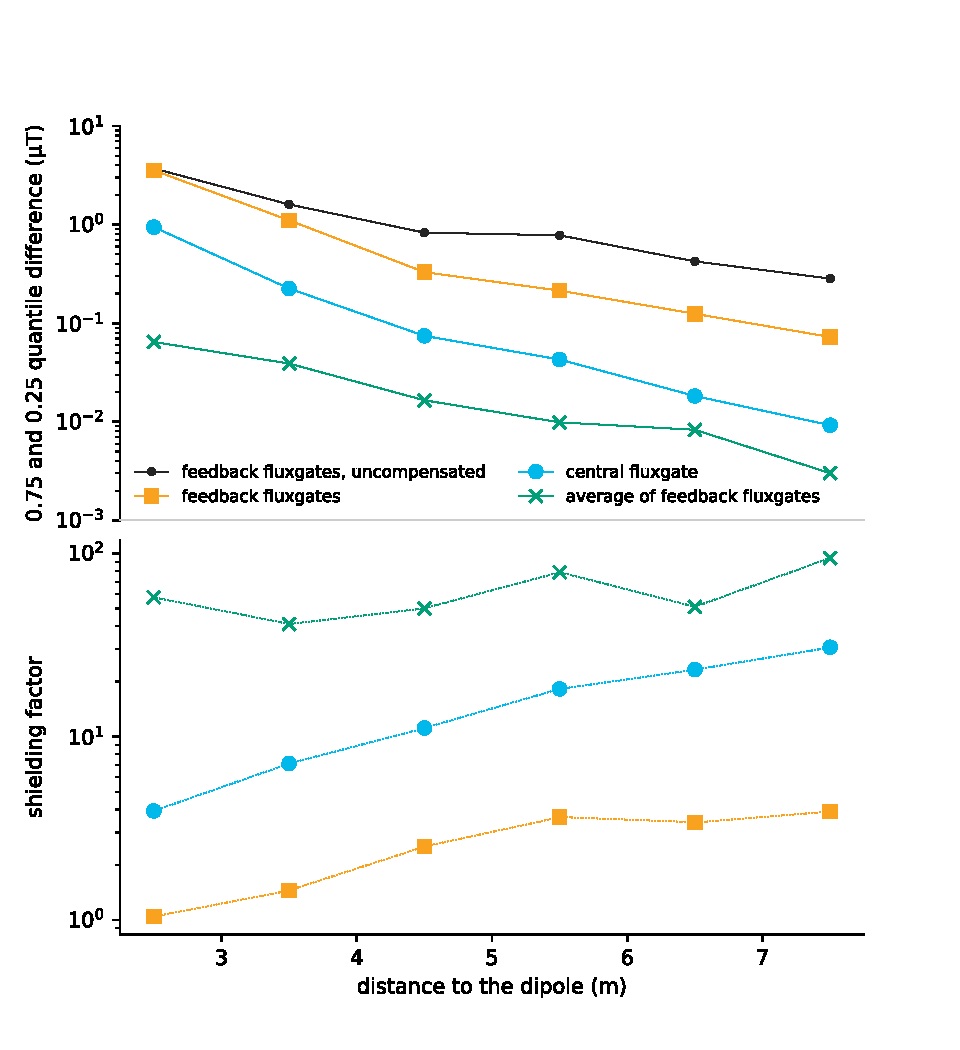
\includegraphics[width=0.85\linewidth]{gfx/prototype/big_magnet_performance_shielding_factor.pdf}
  \caption{Performance of the active shield compensating a dipole disturbance, as a function of the distance away. \emph{Upper part:} the amplitude of the field variations measured as the difference between the 75th and 25th quantiles, uncompensated (black), compensated seen by the feedback sensors (orange), a non-feedback sensor in the centre (blue) and the numerical average of the feedback sensors (green). \emph{Lower part:} the shielding factor, defined as the ratio of the curves in the plot above to the uncompensated variation.}\label{fig:prototype_compensation}
\end{figure}

The amplitude of the variations seen in Fig.\,\ref{fig:prototype_compensation_time} can be quantified as the difference between 75th and 25th quantiles of the readouts.
This measure is plotted in the upper part of Fig.\,\ref{fig:prototype_compensation} as the function of the distance between the dipole disturbance and the centre of the system.
The uppermost black curve is the uncompensated field $\mathbb{B}_0$.
The orange curve below is the compensated field seen by the feedback sensors $\mathbb{B}$ (the bottom part of Fig.\,\ref{fig:prototype_compensation_time}).
We observe that the compensation improved with the distance to the dipole, as the field became weaker and more homogeneous.
In the bottom of the figure the ratio of the two curves, called the \emph{shielding factor}, is plotted in orange.

The next curve (blue) corresponds to the field measured by a sensor placed in the middle of the system.
There the system compensates first-order changes (because they are antisymmetric with respect to the centre).
It suggests that the difference to the shielding factor for the feedback sensors (factor three) can be attributed to the uncompensated variations of first-order gradients.
Furthermore, it suggests that if the system would be extended by a addition of first-order coils, the shielding factor for the feedback sensors (in the whole volume) would be as good as for the centre.

The last curve (green) depicts the variations seen in the average readout of the feedback fluxgates.
An ideal system should compensate it perfectly, regardless of the shape of the field changes.
Yet, the shielding factor for this measure was around 50.
It also did not depend on the distance to the dipole (homogeneity of the field), suggesting that it is a property of the compensation system itself.
The dominant factor is probably the inhomogeneity of the field created by the compensation coils (around \SIrange[range-phrase=--,range-units=single]{1}{2}{\percent}).
Even if the changes of the field were similar in magnitude and pace to the ones discussed, but perfectly homogeneous, this system would not be likely to compensate them better than a factor of 50.




\section{Long-term Stability}
\marginpar{In the PSI environment periods of strong magnetic field changes (tens of microteslas over an hour when nearby magnets ramp) were interleaved with ones of high stability---\SI[detect-all = true]{10}{\nano\tesla} at \SI[detect-all = true]{10}{\second} at night (Fig.\,5.3 in Ref.\,\cite{Franke2013}).}
We have just discussed how the active shield can stabilise the magnetic field in the case of strong variations.
However, the system's internal stability was inevitably finite. In conditions where the environmental magnetic field would be more stable than that, the system would effectively destabilise the field.
In this section we will discuss where the limit of the stability lies.

As the measure of stability we use the \emph{Allan deviation}, a special case of the M-sample variance, defined originally by the Eq.\,11 in Ref.\,\cite{Allan1966}, with $N=2$ and $T = \tau$.
It has a simple interpretation; for a given integration time $\tau$ it calculates the RMS variation from one integrated sample to the next.

\begin{figure}
  \centering
  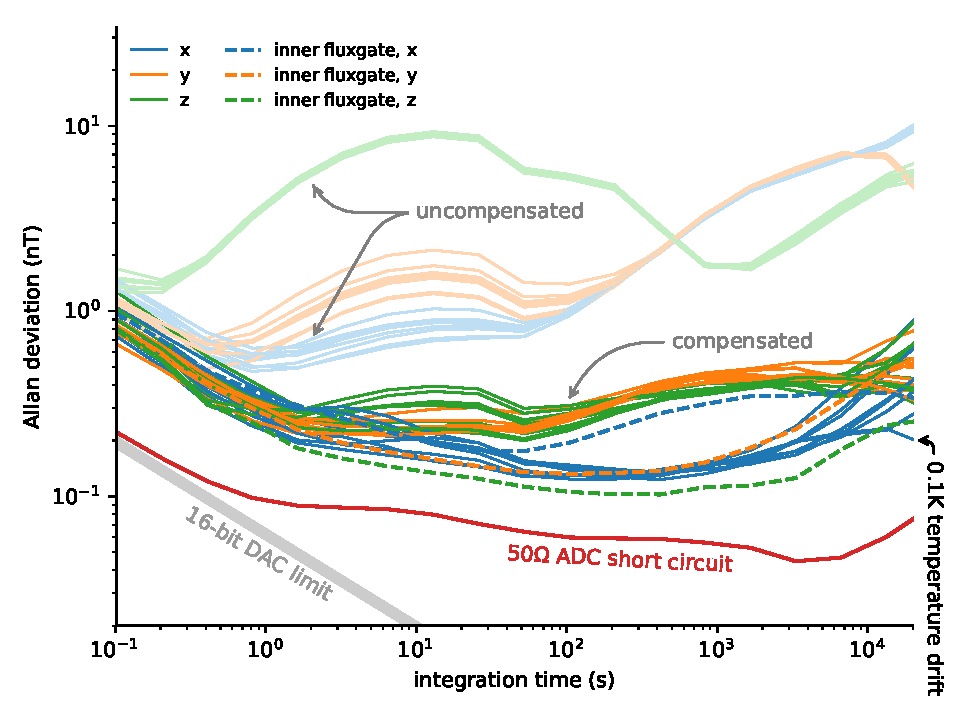
\includegraphics[width=\linewidth]{gfx/prototype/run8_field_stability.pdf}
  \caption{The stability of the active magnetic field compensation.
  The Allan deviation is plotted as the function of integration time.
  The three colours depict the three spatial directions.
  The uppermost three groups of thin, solid lines depict the uncompensated field $\mathbb{B}_0$ measured by the feedback sensors.
  In the dense group of lines below, around \SI{0.3}{\nano\tesla} (corresponding to a temperature stability of \SI{0.1}{\kelvin}, as specified for the fluxgates), are
  the compensated field measured by the feedback sensors $\mathbb{B}$ (solid) and the compensated field measured by a non-feedback fluxgate in the centre of the system (dashed).
  % field measured inside a two layer mu-metal shield (dotted).
  Below that is the stability of the readout of a short-cut ADC channel (red) and the limit set by the quantisation noise of the 16-bit DACs (grey). \note{The lines are impossible to tell apart, make better labels.}}\label{fig:prototype_stability}
\end{figure}

To assess the stability the system ran overnight, with no known activity in the immediate surrounding of the laboratory. The resultant Allan deviation is plotted in Fig.\,\ref{fig:prototype_stability}.
The three uppermost groups of curves depict the stability of the uncompensated field $\mathbb{B}_0$ (as calculated with Eq.\,\ref{eq:uncompensated_field}), at
around \SI{1}{\nano\tesla} for $x$ and $y$, and \SI{10}{\nano\tesla} for $z$. That the stability differed between the spatial components is not a concern---there is no reason to expect the disturbance to be isotropic.
Below, at around \SI{0.3}{\nano\tesla} over a wide range of integration time, is a large group of curves.
Among them are the thick, solid lines depicting the compensated field $\mathbb{B}$.
Even in the most quiet of the conditions in the laboratory the system improved the stability of the field by a factor of two~($x$) to thirty~($z$).

In the previous section it was indicated that in a case of high-order variations, the field in the centre of the system was stabilised better then the one measured by the feedback sensors.
In the Allan standard deviation plot the stability of the sensor in the centre is depicted with dashed lines;
they lie in the large group around \SI{0.3}{\nano\tesla},
% although rather on its lower side,
suggesting that the variations during the measurement were homogeneous.

% Why was the improvement not better? In the plot there seems to be a fixed limit for the stability. Another set of curves, the dotted ones, provide a hint. They depict the stability of the field observed with an additional sensor mounted inside a two-layer mu-metal shield, which should provide a factor of a hundred in shielding (the second layer was a cylinder without end caps aligned with the $z$-axis of the sensor, hence the worse performance in this direction). Yet, the registered stability is no better than that of the active stabilisation system.

Why was the improvement not better?
The limit came most likely from the temperature drifts.
According to the specification of the Stefan Mayer Instruments sensor (FLC3--70), thermal drifts of \SI{2}{\nano\tesla\per\kelvin} can be expected,
meaning the the observed stability corresponds to temperature stability as small as \SI{0.1}{\kelvin}.
Even at night the temperature in a non-temperature-stabilised laboratory cannot be expected to be more stable than this.
This limit can be pushed a factor twenty lower with higher-quality (and more expensive) sensors.
Commercially available Stefan Mayer Instruments FL1--100 and Bartington Mag-03 are specified to drift \SI{0.1}{\nano\tesla\per\kelvin} with a $\SI{\pm 100}{\micro\tesla}$ measuring range.

However, there is an other limitation.
Figure\,\ref{fig:prototype_stability} features a red line labeled ``\SI{50}{\ohm} ADC shortcut''.
This is the stability of the readout of an ADC channel with the terminals connected with a \SI{50}{\ohm} resistor.
Even if the magnetic field sensors would have output a perfectly stable voltage, the digitised information would be no more stable than this.
A higher class digitisers could perform better.

Interestingly, the stability was fully defined by the measurement chain: the sensors and the digitisers.
Instabilities of the output chain, DACs and amplifiers, indistinguishable from changes in the magnetic field, were corrected by the system itself.
One exception is the discrete nature of the currents that can be applied.
The lowest curve on the plot is the limit on the stability due to the bit depth of the DACs. A quantisation resolution $\Delta$ corresponds to white noise with an RMS amplitude $\Delta / \sqrt{12}$ (derived for example in Sec.\,IV.A in Ref.\,~\cite{Gray1998}).
This noise then scales down as $\tau^{-1/2}$ with the integration time.
The system's 16-bit DACs had $2^{16}$ levels mapped onto a $\SI{\pm 100}{\micro\tesla}$ range.
This defines the quantisation at the feedback time of inverse $\SI{200}{\hertz}$.
In total the limit from the quantisation at the integration time $\tau$ is
\begin{equation}
  \frac{ \SI{200}{\micro\tesla} }{ 2^{16} \ \sqrt{12} \ \sqrt{ \SI{200}{\hertz}\ \tau} } \ .
\end{equation}
Aside from the obvious---increasing the bit depth of the DACs---this limit can be pushed further by increasing the feedback frequency or decreasing the range of the operation.




\section{Open-design cage}
The disadvantage of the first-iteration design was that the cage was fully closed, making installation or removal of large items inside essentially impossible.
In particular, the active magnetic shield at ETH could, in future, be used in combination with a mu-metal shield inside it.

The solution was to modify the system in way that one of the faces would hold no wires at all.
As neither the coil design method (Ch.\,\ref{ch:coil_design}) nor its implementation are restricted to regular grids, it could be fully realised within the framework.
In the scope of this work coils corresponding to the cartesian harmonic polynomials $n = 1, \ldots, 8$ (Tab.\,\ref{tab:coils_cartesian_harmonics}) were designed and the $y$-coil ($n = 2$) was wound and mapped.
The face that was left open is square (the one to the left in Fig.\,\ref{fig:prototype_photo}).

% This solution had the immediate advantage of demonstrating the power of the coil design method. The next iteration is designed with one face (rectangular one, $Y-$) left open. Designed fully following the algorithm.

\begin{figure}
  \centering
  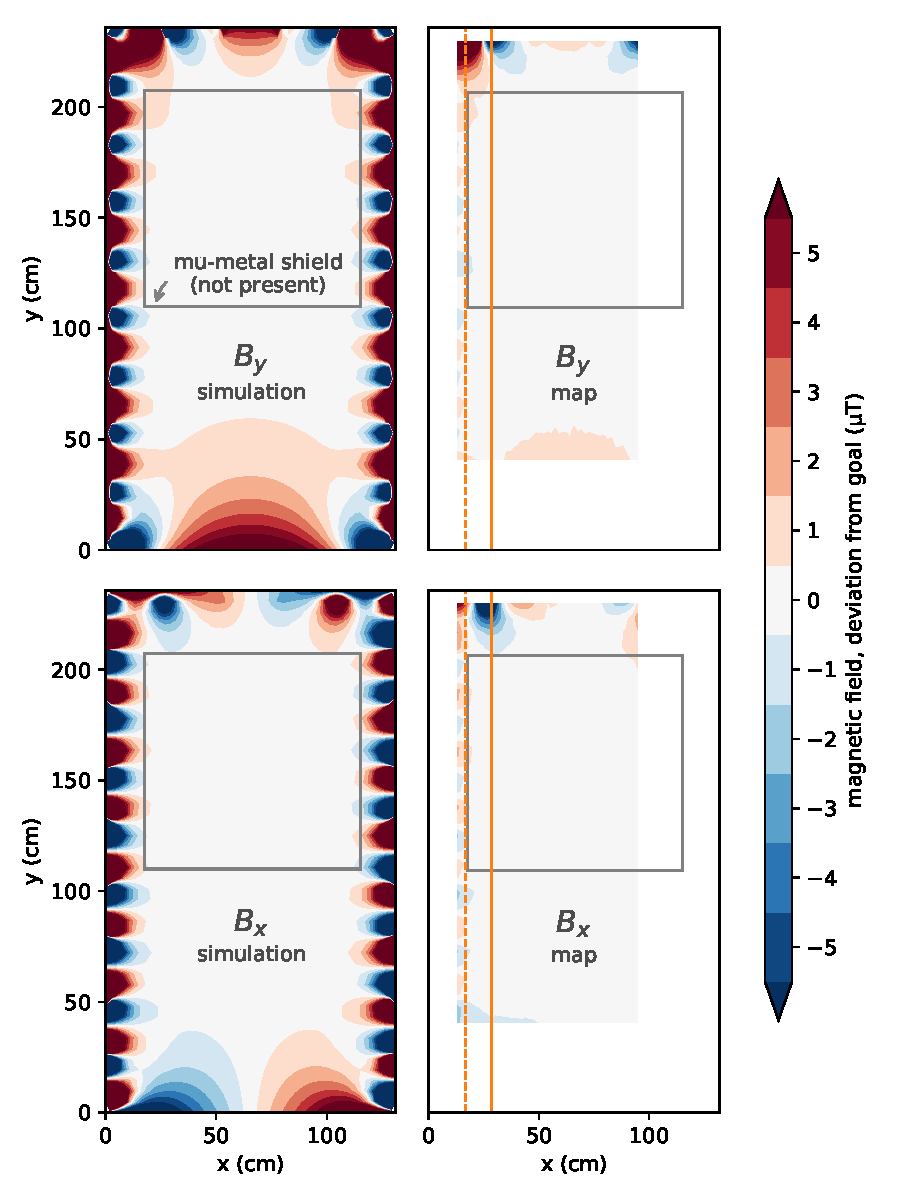
\includegraphics[width=\linewidth]{gfx/prototype/open_planar_map_comparison.pdf}
  % 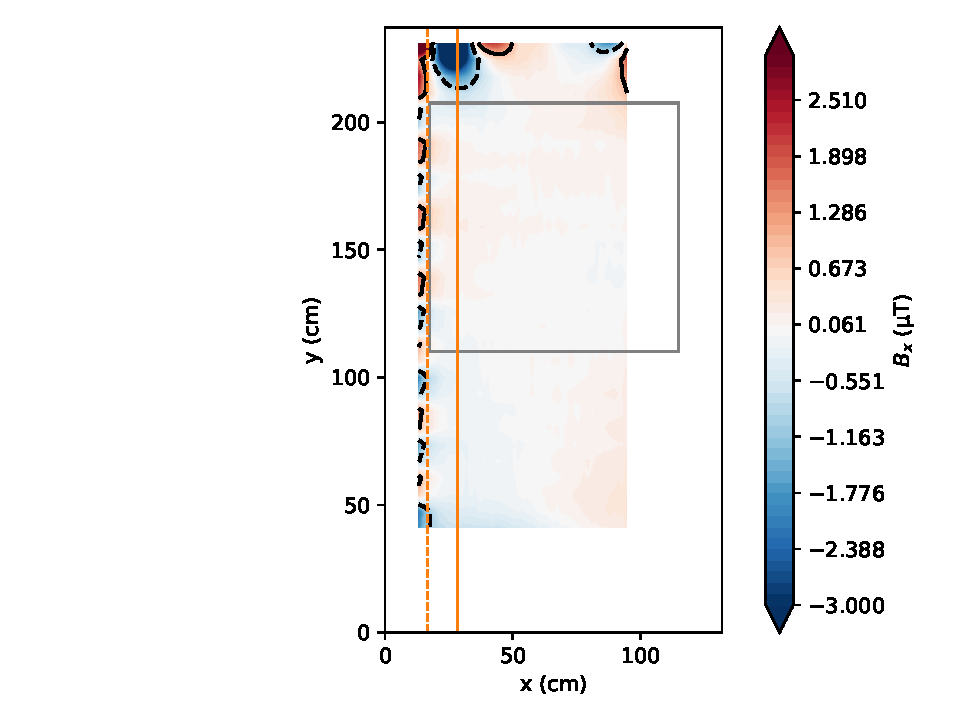
\includegraphics[width=0.45\linewidth,trim={5cm 0 0 0},clip]{gfx/prototype/open_planar_map_Y_Bx.pdf}\quad
  % 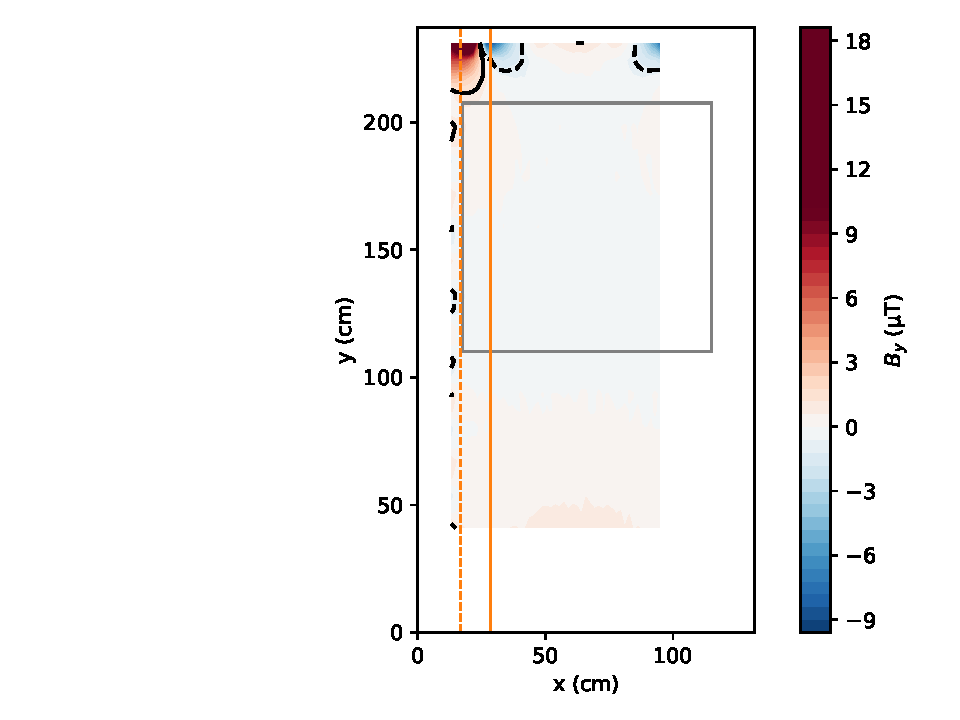
\includegraphics[width=0.45\linewidth,trim={5cm 0 0 0},clip]{gfx/prototype/open_planar_map_Y_By.pdf}
  \caption{The simulations (left column) and maps (right column) of the field of the $y$-coil. In the bottom row the $x$ component of the field is shown, in the top row: the $y$ component. The latter relative to the goal value of \SI{50}{\micro\tesla}. The contour of a mu-metal shield intended to be put in the system is depicted. To account for misalignments of the sensor, the map has been normalised to the average field measured in the middle region of highest homogeneity. The mapped field along the vertical orange lines is plotted in Fig.\,\ref{fig:prototype_open_design_Ycoil_map_section}.}\label{fig:prototype_open_design_Ycoil_maps}
\end{figure}

\begin{figure}
  \centering
  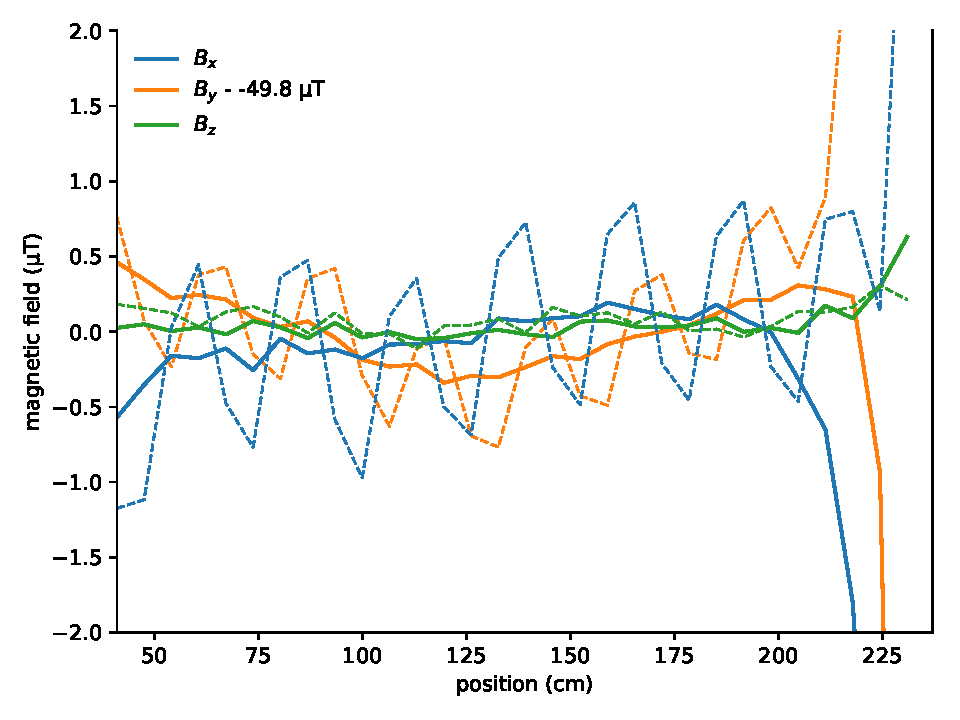
\includegraphics[width=\linewidth]{gfx/prototype/open_planar_map_Y_By_section.pdf}
  \caption{The measured field of the $y$-coil along the solid and dashed lines depicted in Fig.\,\ref{fig:prototype_open_design_Ycoil_maps}. The thin, dashed lines depict the field \SI{16.6}{\centi\metre} away from the surface of the coils in the $x$ direction (the fiducial volume was \SI{15.5}{\centi\metre} away). The thick, solid lines correspond to a distance of \SI{28.5}{\centi\metre}away. The vertical line on the right depicts the surface of the coils along $y$.}\label{fig:prototype_open_design_Ycoil_map_section}
\end{figure}

In Fig.\,\ref{fig:prototype_open_design_Ycoil_maps} both simulations and maps of the field of the $y$ coil are shown.
\marginpar{In the whole fiducial volume the homogeneity was predicted to be stricly better than~\SI[detect-all=true]{4}{\percent}.}
In these simulations the homogeneity was predicted to be \SI{2}{\percent} (\SI{1}{\micro\tesla} in the \SI{50}{\micro\tesla} field in the figure) in the $97.5 \times 97.5 \times \SI{97.5}{\centi\metre}$ volume (depicted in grey the figure).
This volume would be occupied by a cubic mu-metal shield intended to be put in the system.
The measured field, mapped as described in Sec.\,\ref{sec:prototype_mapping}, confirms that the homogeneity could be achieved in practice.
Figure~\ref{fig:prototype_open_design_Ycoil_map_section} details the measured field along the orange lines marked in Fig.\,\ref{fig:prototype_open_design_Ycoil_maps}.

% The simulation of the field produced by the optimal design of the $y$-coil is presented in the upper part of Fig.\,\ref{fig:prototype_open_design_Ycoil_maps}. On the left-hand side the deviation of the $x$ component from zero is shown, on the right-hand side: one of the $y$ component from \SI{50}{\micro\tesla}. In the bottom of the figure a map of the two components is plotted. Additionally, two sections of the map, along the vertical lines depicted in orange, are presented in Fig.\,\ref{fig:prototype_open_design_Ycoil_map_section}. The dashed line is xxx away from the surface of the coils and corresponds to the edge of the fiducial volume. The design fully meets the specification of \SI{2}{\percent} homogeneity in the fiducial volume.

% and the map of the $y$-coil are presented in Fig.\,\ref{fig:prototype_open_design_Ycoil_maps}. In Fig.\,\ref{fig:prototype_open_design_Ycoil_map_section} the section along the $y$ direction is plotted.
% Now some thoughts about it. We see, that it behaves exactly as expected. For now the colours are inverted.

% \note{It is now a bit weird, that I have a detailed wiring plan for the $x$-coil, but I write more about the $y$-coil (the one I have)}.

\begin{figure}
  \centering
  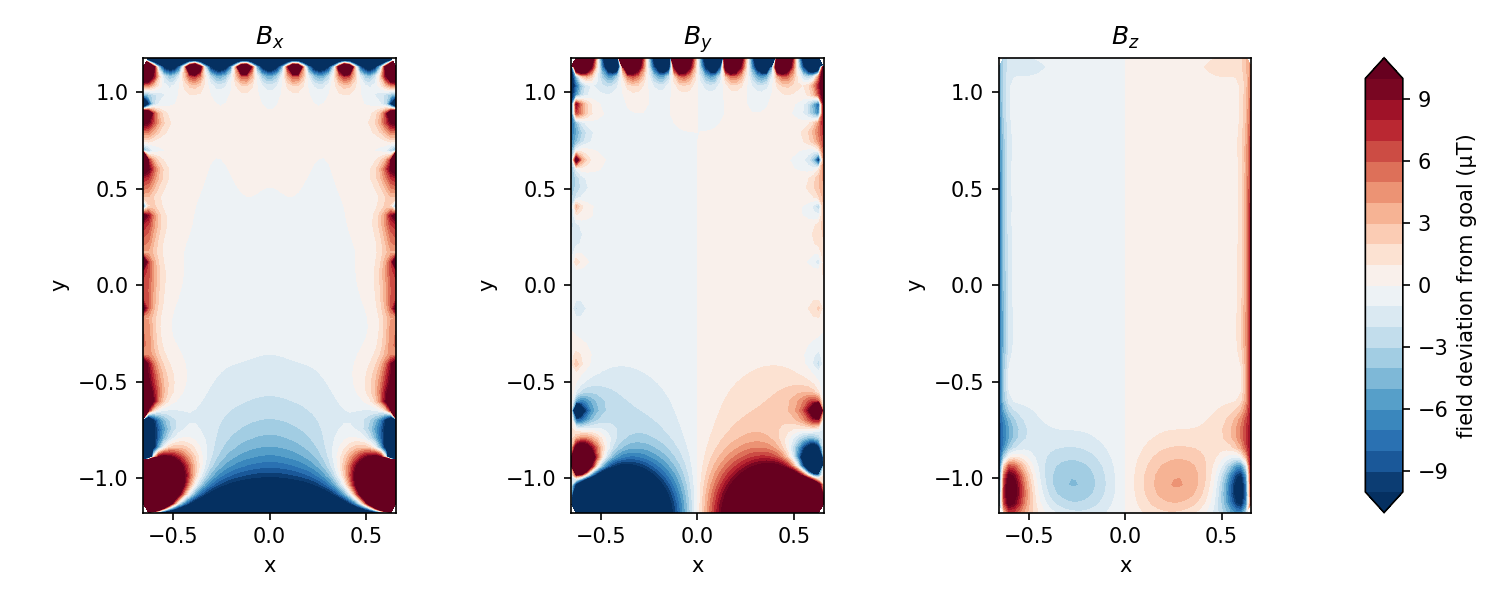
\includegraphics[width=\linewidth]{gfx/prototype/open_design_Xcoil_field_XY_z0_33.png}
  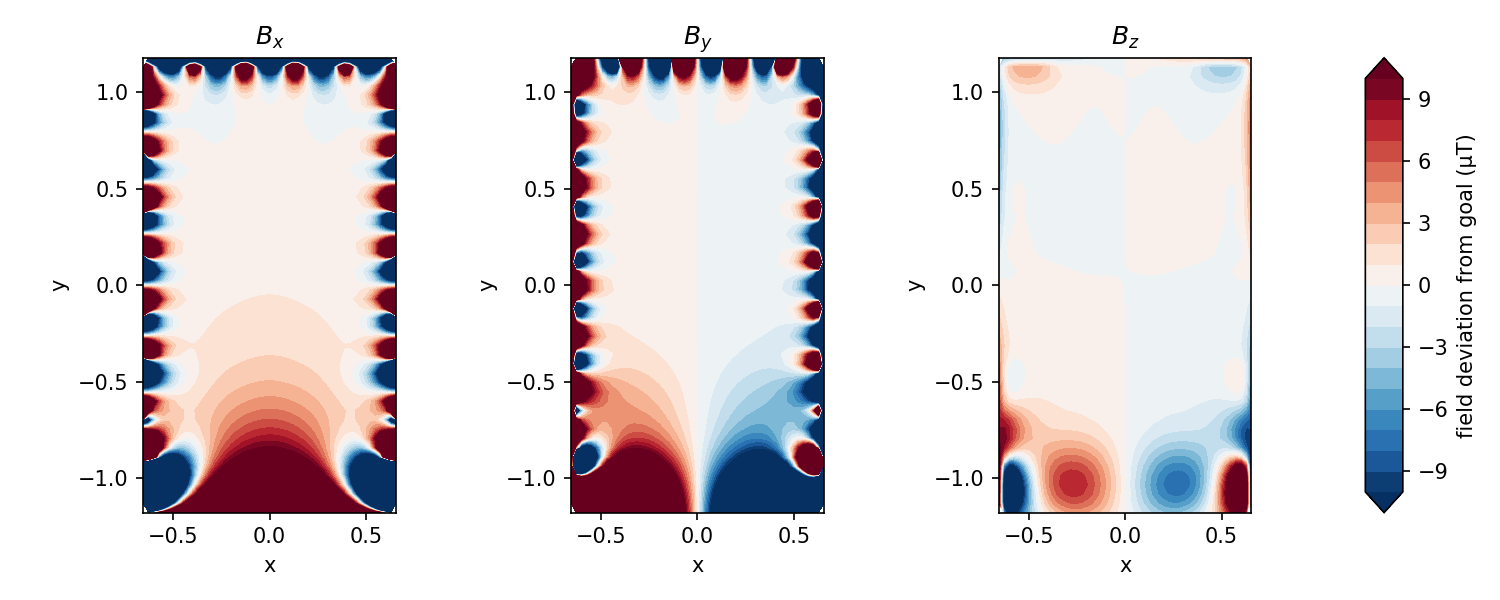
\includegraphics[width=\linewidth]{gfx/prototype/open_design_n5coil_field_XY_z0_33.png}
  \caption{Simulation of the open-design cage for $n = 1$ ($x$-coil, top) and the $n = 5$ (linear gradient, bottom).
  The colour depicts the deviation of the coil, $x$, $y$ and $z$ components, from the target field.
  The section in the XY plane at height $z=\SI{33}{\centi\meter}$ is shown.
  The open face is at the bottom of the plots.
  \note{Improve this figure still, make it similar to Fig.\,\ref{fig:prototype_open_design_Ycoil_maps}.
  Remove unnecessary axis ticks, only one colour-bar, adjust the colour scale not to have a sharp transition exactly at zero.}}\label{fig:prototype_open_design_simulation}
\end{figure}

\begin{figure}
  \centering
  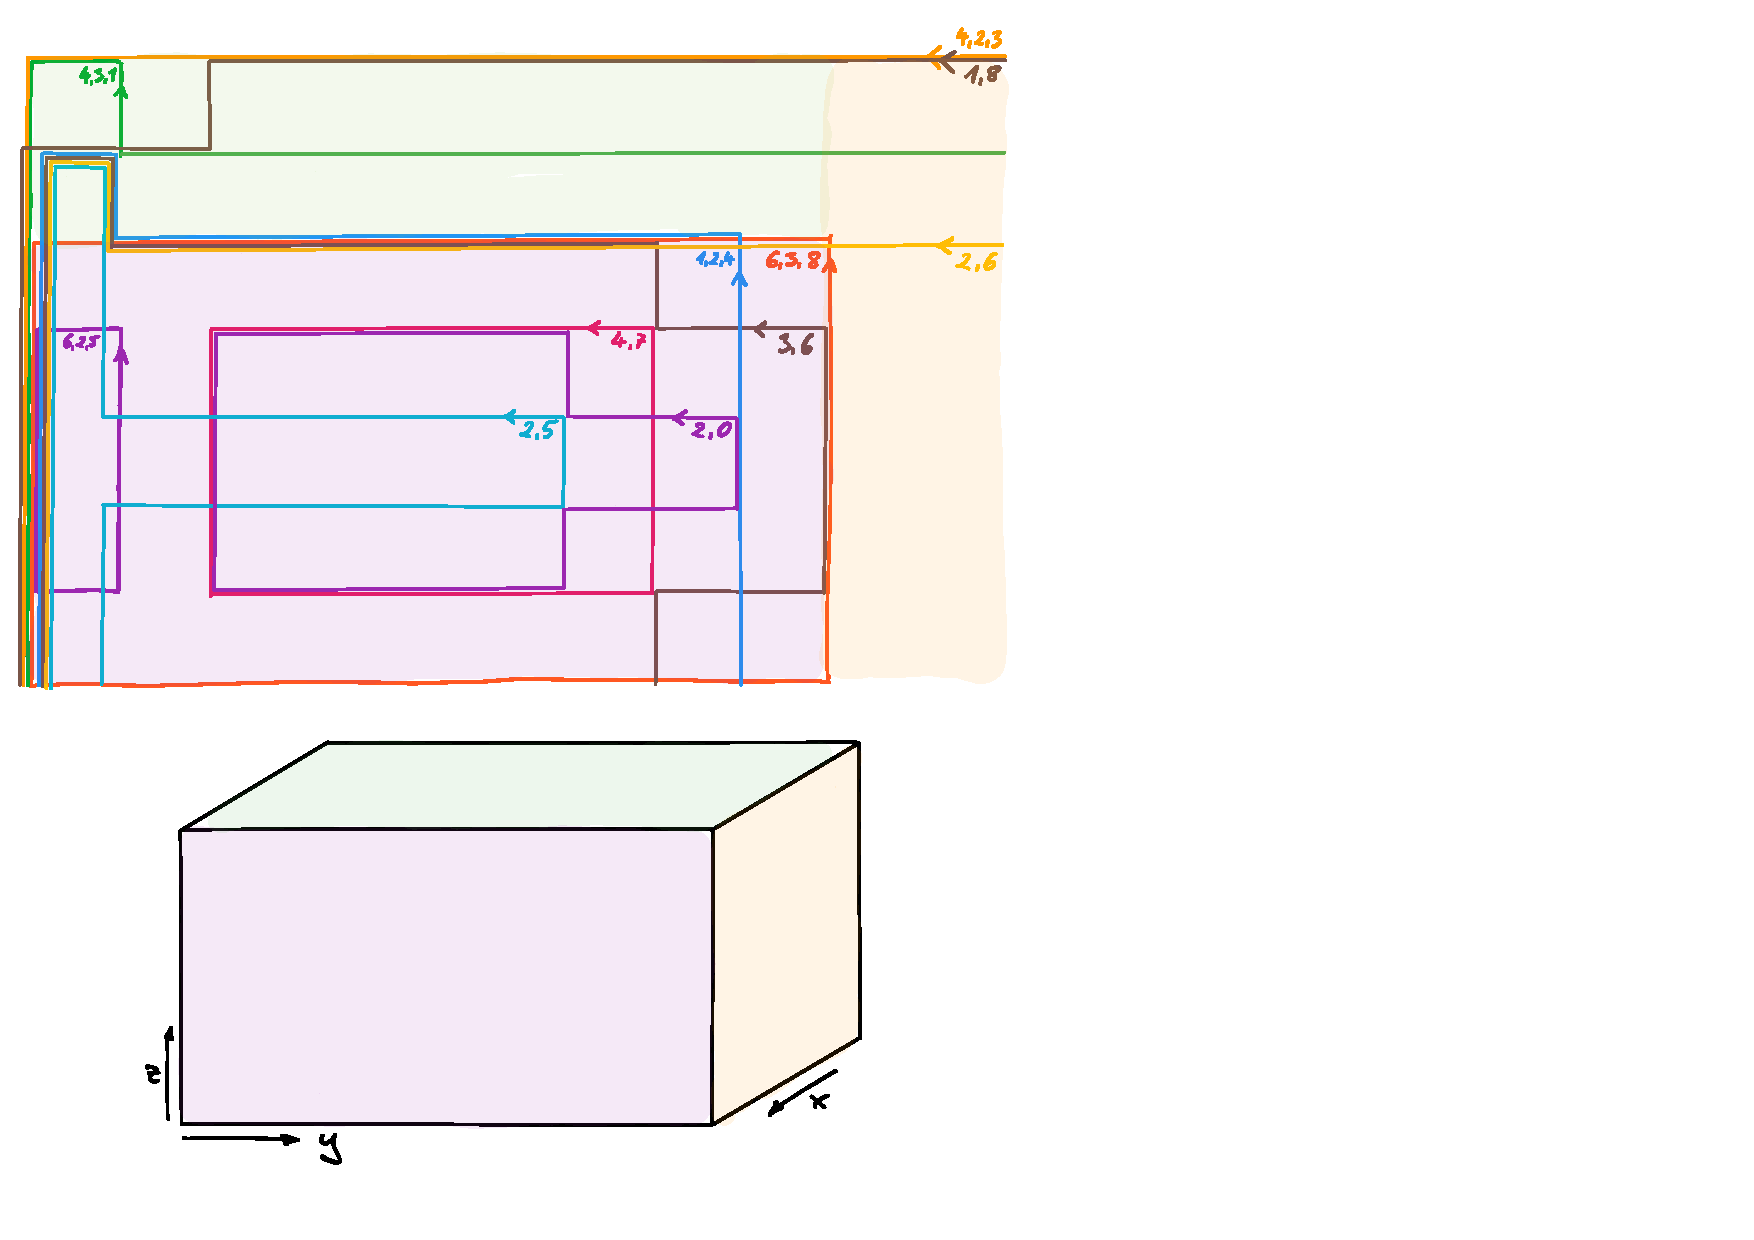
\includegraphics[width=\linewidth]{gfx/prototype/open_design_Xcoil_coils.pdf}
  \caption{The first 22 (out of 64) loops of the $x$-coil in the open-design cage. For each loop the digits indicate the number of \SI{5}{\ampere}, \SI{1}{\ampere} and \SI{0.1}{\ampere} windings (per \SI{50}{\micro\tesla} field, leading zeros are omitted).
  Half of the cage is flattened out, the other being identical on symmetry grounds.
  The open face is located to the left. The faces have been coloured to help with orientation.}\label{fig:prototype_open_design_Xcoil_coils}
\end{figure}

The remaining seven coils were designed.
Winding them, however, was beyond the scope of this work.
The simulated field produced by the optimal designs for the $n = 1$ ($x$-coil) and the $n = 5$ coil (Tab.\,\ref{tab:coils_cartesian_harmonics}) are presented in Fig.\,\ref{fig:prototype_open_design_simulation}.
Despite lack of one face in the grid, the field is reproduced in a volume large enough to fit the mu-metal cube, even in the case of the linear-gradient coil.
In Fig.\,\ref{fig:prototype_open_design_Xcoil_coils} the first 22 (out of 64) loops of the $x$-coil are depicted.
Note in particular the high density of the cables along the edges of the open face.
% Except the part near the open face (at the bottom of the plots) the field in the volume is reproduced in the whole fiducial volume down to \SI{2}{\percent} (\SI{1}{\micro\tesla} on a \SI{50}{\micro\tesla} field), even for the gradient coil.
% Fig.\,\ref{fig:prototype_open_design_Xcoil_coils} shows the first 22 (out of 64) current loops of the $x$ coil.
%\note{All with 1A wires? not much more} The numbers show the number of windings in the 5A, 1A and 0.1A scheme.

% \note{Here I could mention how inhomogeneous was the field in the lab. I.e.\ how much field was still left when running the homogeneous compensation. This would motivate the need for the linear gradient coils.}

% The calculation with the fiducial volume of\ldots done for homogenous and 1st gradient coils. Fig.\,\ref{fig:prototype_open_design_simulation} presents the sections for\ldots Fig.\,\ref{fig:prototype_open_design_Xcoil_coils} shows the first 22 (out of 64) current loops. \note{All with 1A wires? not much more} The numbers show the number of windings in the 5A, 1A and 0.1A scheme.

The open-design $y$-coil was a significant step forward from the closed-cage design.
It has been demonstrated that the coil design framework is capable of handling irregular grids, and the designs can be successfully realised in practice.
While the prototype at ETH could be further extended by winding the remaining seven coils, the positive results of the $y$-coil already supported the case for designing a system for the n2EDM experiment.




\section{n2EDM design}
Let us recall the discussion in Sec.\,\ref{sec:n2EDM_challenges} on the design challenges of an active magnetic field compensation system for the n2EDM experiment.
The main point of concern were the spatial constraints.
Firstly, there would not be much space available around the mu-metal shield, calling for a coil system with a large fiducial volume.
Secondly, only an irregular cage would avoid collisions with other components of the experiment and facilities in the hall.

\begin{figure}
  \centering
  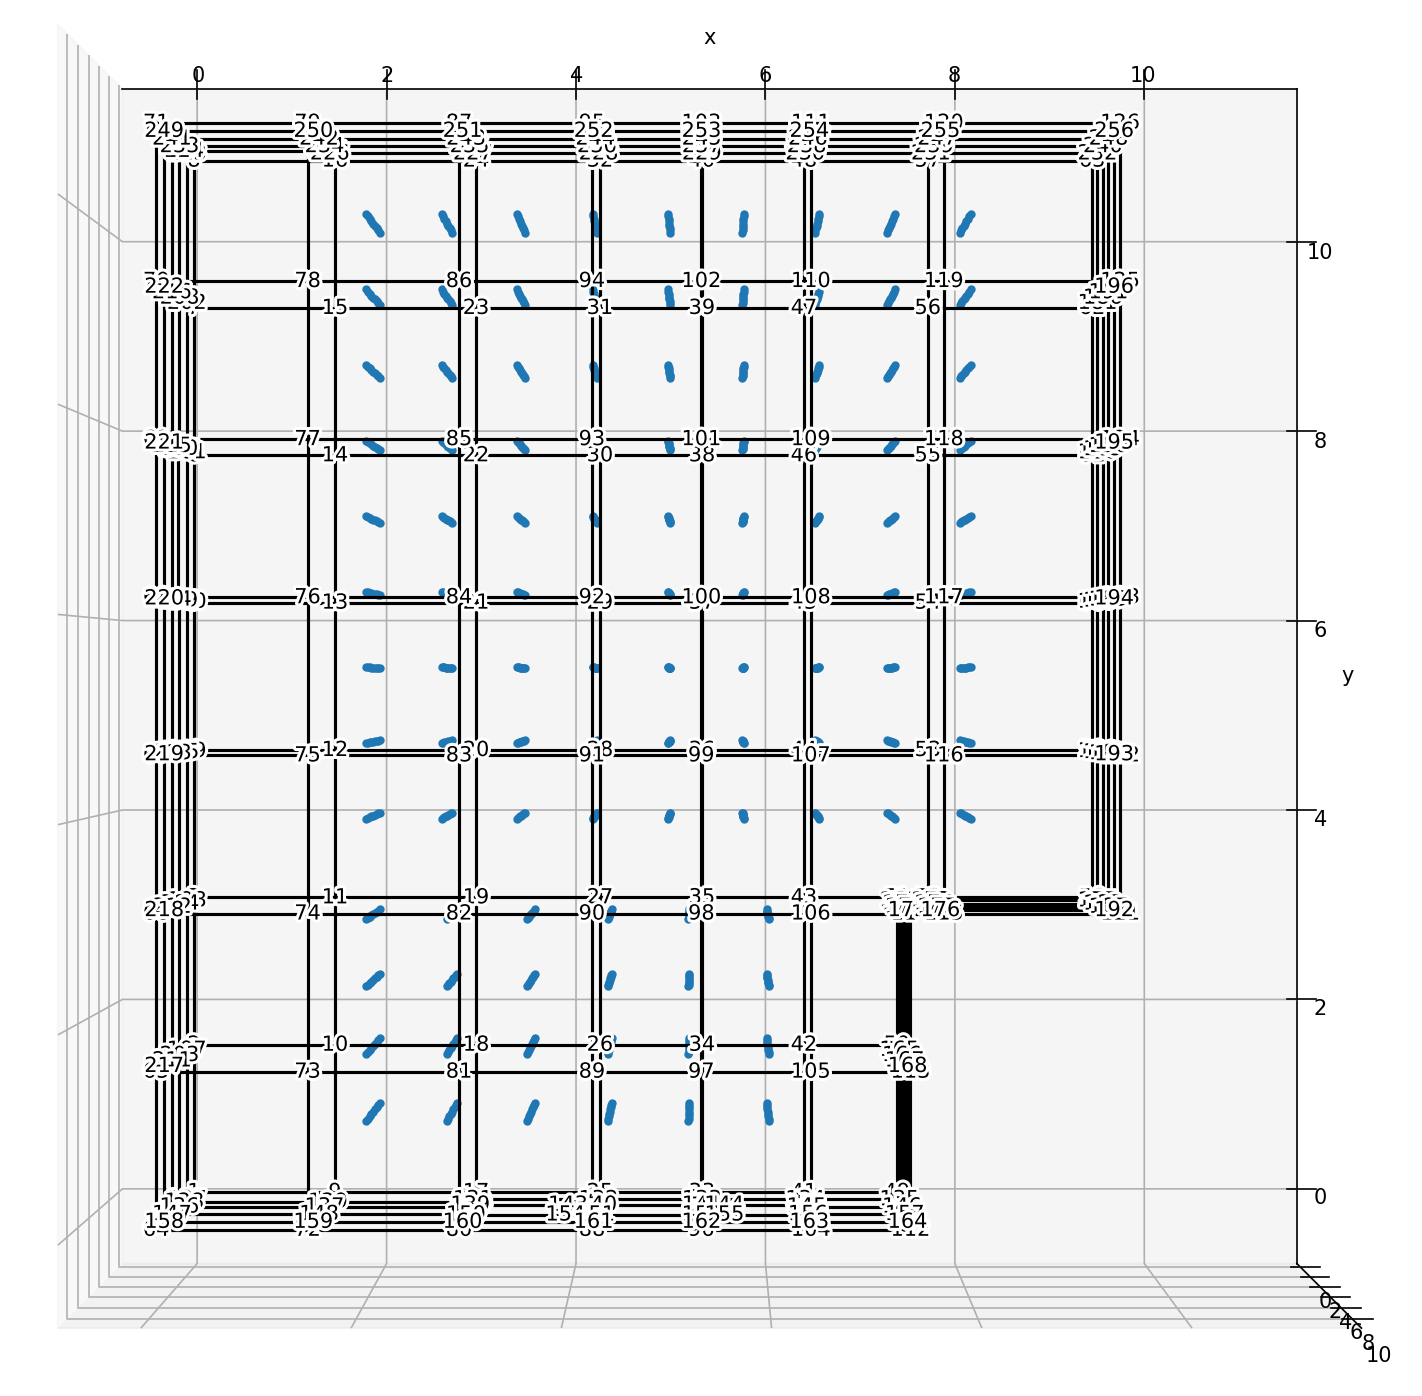
\includegraphics[width=\linewidth]{gfx/prototype/n2EDM_system_top.png}
  \caption{A computer model of the n2EDM active magnetic shield cage. Replace with a better figure showing the design\ldots The best show the front face, too.}\label{fig:n2EDM_design_top}
\end{figure}

A cage for the compensation coils was incorporated in an existing CAD model of the experiment.
It was composed out of rectangles around \SI{1.5}{\metre} large.
Care has been taken to avoid conflicts with other parts of the apparatus.
The cage, depicted in Fig.\,\ref{fig:n2EDM_design_top}, was then implemented in the coil-design framework.

\begin{figure}
  \centering
  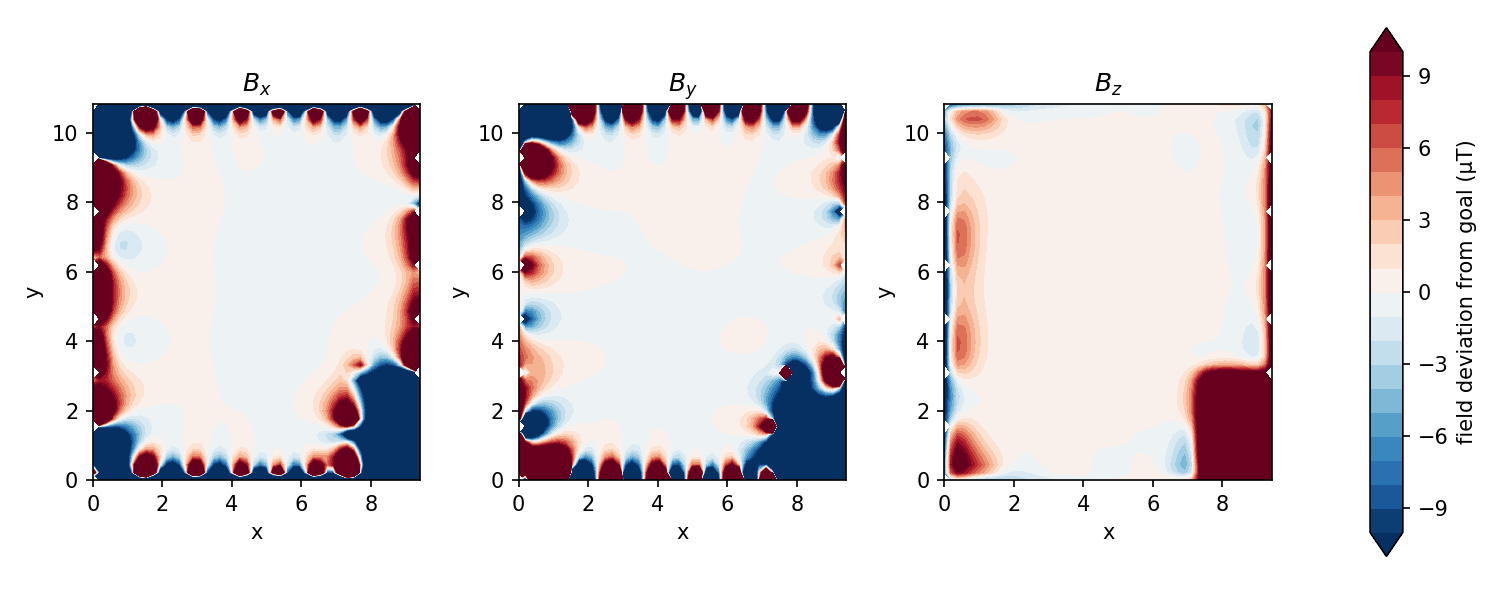
\includegraphics[width=\linewidth]{gfx/prototype/n2EDM_field_Xcoil_XY_z6_4.png}
  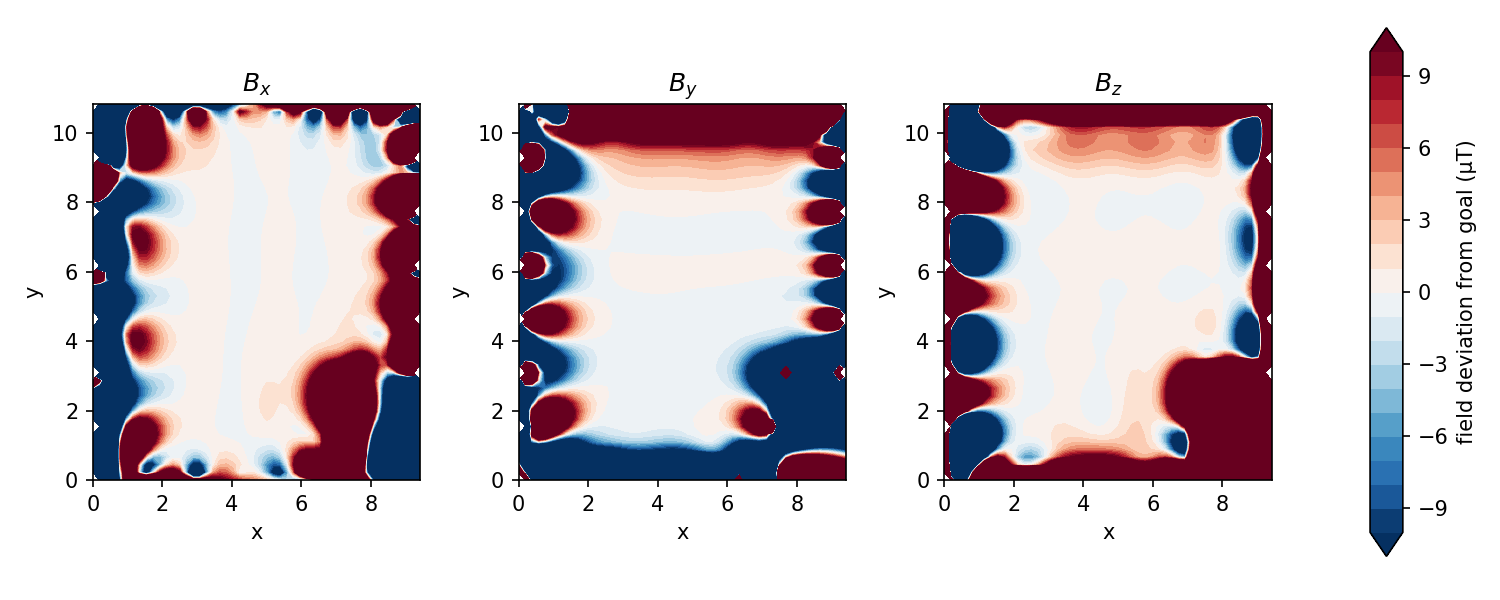
\includegraphics[width=\linewidth]{gfx/prototype/n2EDM_field_n6coil_XY_z6_4.png}
  \caption{Simulation of the n2EDM design.
  The colour represents the deviation from the target field, for the $x$, $y$ and $z$ components of the field.
  The section in the XY plane at height $z=\SI{6.4}{\meter}$ is shown.
  The open face is at the bottom of the plots.
  Top: Depiction of a coil designed to produce a homogeneous field along $x$ (left-to-right on the plot).
  Bottom: $n=6$ gradient (see some table somewhere)\ldots \note{Mark the contour of the shield. Make it similar to Fig.\,\ref{fig:prototype_open_design_Ycoil_maps}.
  Also, normalise so that the magnitude of the field matches what is shown in the histogram.}}\label{fig:n2EDM_design_fields}
\end{figure}

\begin{figure}
  \centering
  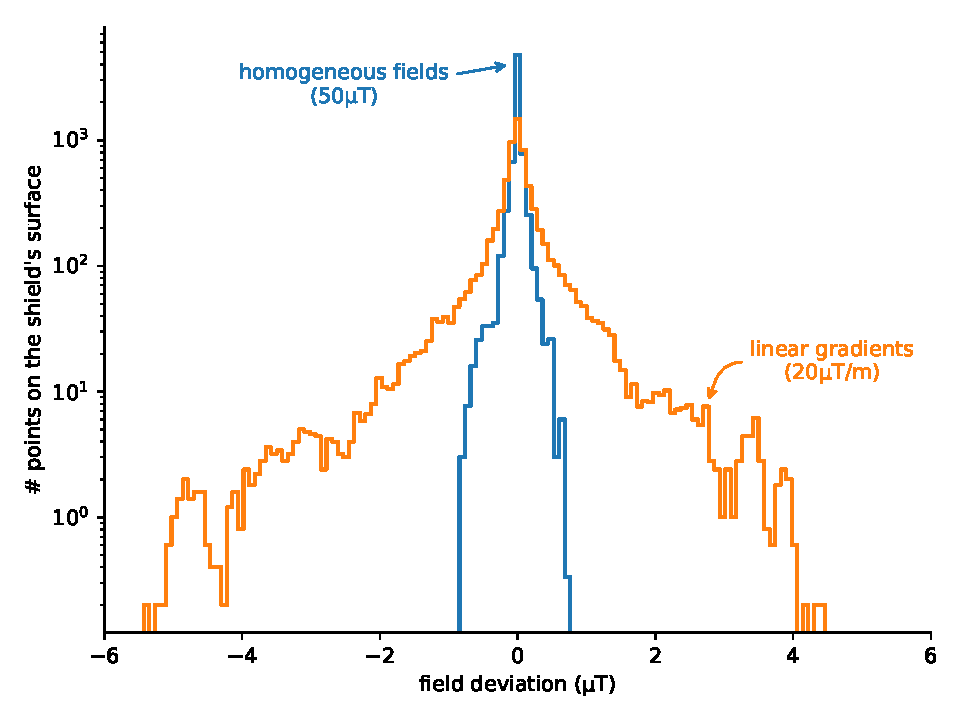
\includegraphics[width=\linewidth]{gfx/prototype/n2EDM_coils_field.pdf}
  \caption{The quality of the field produced by the designed coils for the n2EDM experiment, quantified by a histogram of the deviation of the design's simulated field from the target one, as measured on the surface of the mu-metal shield.
  One entry corresponds to a difference in one spatial direction at one point.
  The designs for the homogeneous coils have been averaged as they are similar. The deviations for the linear gradients were also averaged.
  \note{Check once again the height of the MSR above the floor.}}\label{fig:n2EDM_design_deviation}
\end{figure}

A set of coils has been designed for the first eight cartesian harmonics (Tab.\,\ref{tab:coils_cartesian_harmonics}).
The field simulated for a $n = 1$ homogeneous field coil and a $n = 6$ linear gradient are depicted in Fig.\,\ref{fig:n2EDM_design_fields}.
The contour of the n2EDM mu-metal shield is depicted in grey.
The quality of the field, as simulated on the surface of the mu-metal shield, is plotted in Fig.\,\ref{fig:n2EDM_design_deviation}.
The deviation from the pure harmonics is shown.
The magnitude of the fields was chosen to be roughly the expected compensation values.
% : \SI{50}{\micro\tesla} field for the homogeneous components and \SI{20}{\micro\tesla\per\metre} for the linear gradients.
\marginpar{The magnitudes of homogeneous fields and gradients have different units.
They can only be compared given a characteristic length,
in this case the size of the active shield.}
When cancelling a perfectly homogeneous \SI{50}{\micro\tesla} field the remnant is expected to be $< \SI{1}{\micro\tesla}$ (which corresponds to \SI{2}{\percent}).
In the case of a \SI{20}{\micro\tesla\per\meter} linear gradient the remnant would be $< \SI{6}{\micro\tesla}$ (\SI{6}{\percent} for the \SI{5}{\metre} large shield).

Remnant fields this small are unlikely to be a limiting factor in the dynamic stabilisation; recall the discussion at the end of Sec.\,\ref{sec:dynamic_stabilisation}, in particular Fig.\,\ref{fig:prototype_compensation}.
The ability of the prototype to actively shield was limited by the inhomogeneity of the field changes.
The homogeneity in the zeroth order coils for the n2EDM active shield's design was comparable to the ones of the prototype: \SIrange[range-phrase=--,range-units=single]{1}{2}{\percent}.
Therefore, the limit in the shielding factor was expected to be similar at around 50.

In the design the limiting factor was identified to be the inability of the active shield's coils to reproduce the field changes.
It was then crucial to characterise the changes in the experimental site, so that appropriate coils could be built.
The characterisation is the topic of the next chapter.




\section*{Next-generation active magnetic shielding -- Conclusion}
% What is new about the next-generation active magnetic field compensation?
Active magnetic shields built on a grid can easily deal with spatial constrains.
The grid is shared between different coils, making it easy to overlay a number of them.
In particular, it is possible to construct coils for the mutually orthogonal terms of the cartesian harmonic expansion of the field.
This simplifies the control of the system.

% What have I done, how successful was it?
An active shield built at ETH demonstrated the grid-based approach.
Maps of the coils confirmed that the \SI{1310}{\milli\metre} large coils achieve a \SI{2}{\percent} homogeneity in a \SI{1000}{\milli\metre} large volume.
The prototype showed the practical advantages of using cable channels as a support structure for the coils.
The shield performed well when compensating a strong, nearby dipole source.
Even in magnetically quiet conditions, the stability of the field was further improved down to \SI{0.3}{\nano\tesla} in timescales from seconds to hours.

In the second iteration the coils were designed with one face of the cage left open.
This made the designs of the coils significantly more complicated.
The maps of an open-design coil demonstrated its adherence to the simulated design.

Finally, a design of an active magnetic shielding cage for the n2EDM experiment was proposed.
Thanks to the flexibility of the grid-based approach a design could fully respect the tight spatial constraints.
Despite the complicated geometry, it is expected to perform similarly to the small-scale prototype.
